\section{Ergebnisse / Evaluation}
%%%%%%%
% http://www.caps.in.tum.de/himmuc/
% Datenerhebenung (+ auf himmuc!) -> Max
% Skalierungs bzgl anzahl an nodes
% Vergleich OpenMP und mehrere MPI pro Node -> Tobi
% Overhead durch Balancer -> Florian
% Overhead durch MPI / Websocket / DrawTiles (konstant)
% Vergleich SIMD / Rohcode -> Niels

% Nutzbarkeit/ HCI -> Max
% vergleich x86 -> Max
% \subsection{Performanzerhöhung alternative Parallelisierungsmechanismen}

\subsection{Datenerhebung}
% Max
% Datenerhebung auf himmuc cluster
% Messen der Timings im backend (Wie kommen die Daten im frontend zu stande?)
% Auswahl der repräsentativen Punkte
% Grobes Intro zu der folgenden Evaluation
\begin{figure}
	\centering
	\begin{tabular}{ccc}
		Außerhalb                                                  & Randregion                                                    & Innerhalb                                                 \\
		\hline
		
\includegraphics[width=0.2\textwidth]{img/Evaluation/out1} & 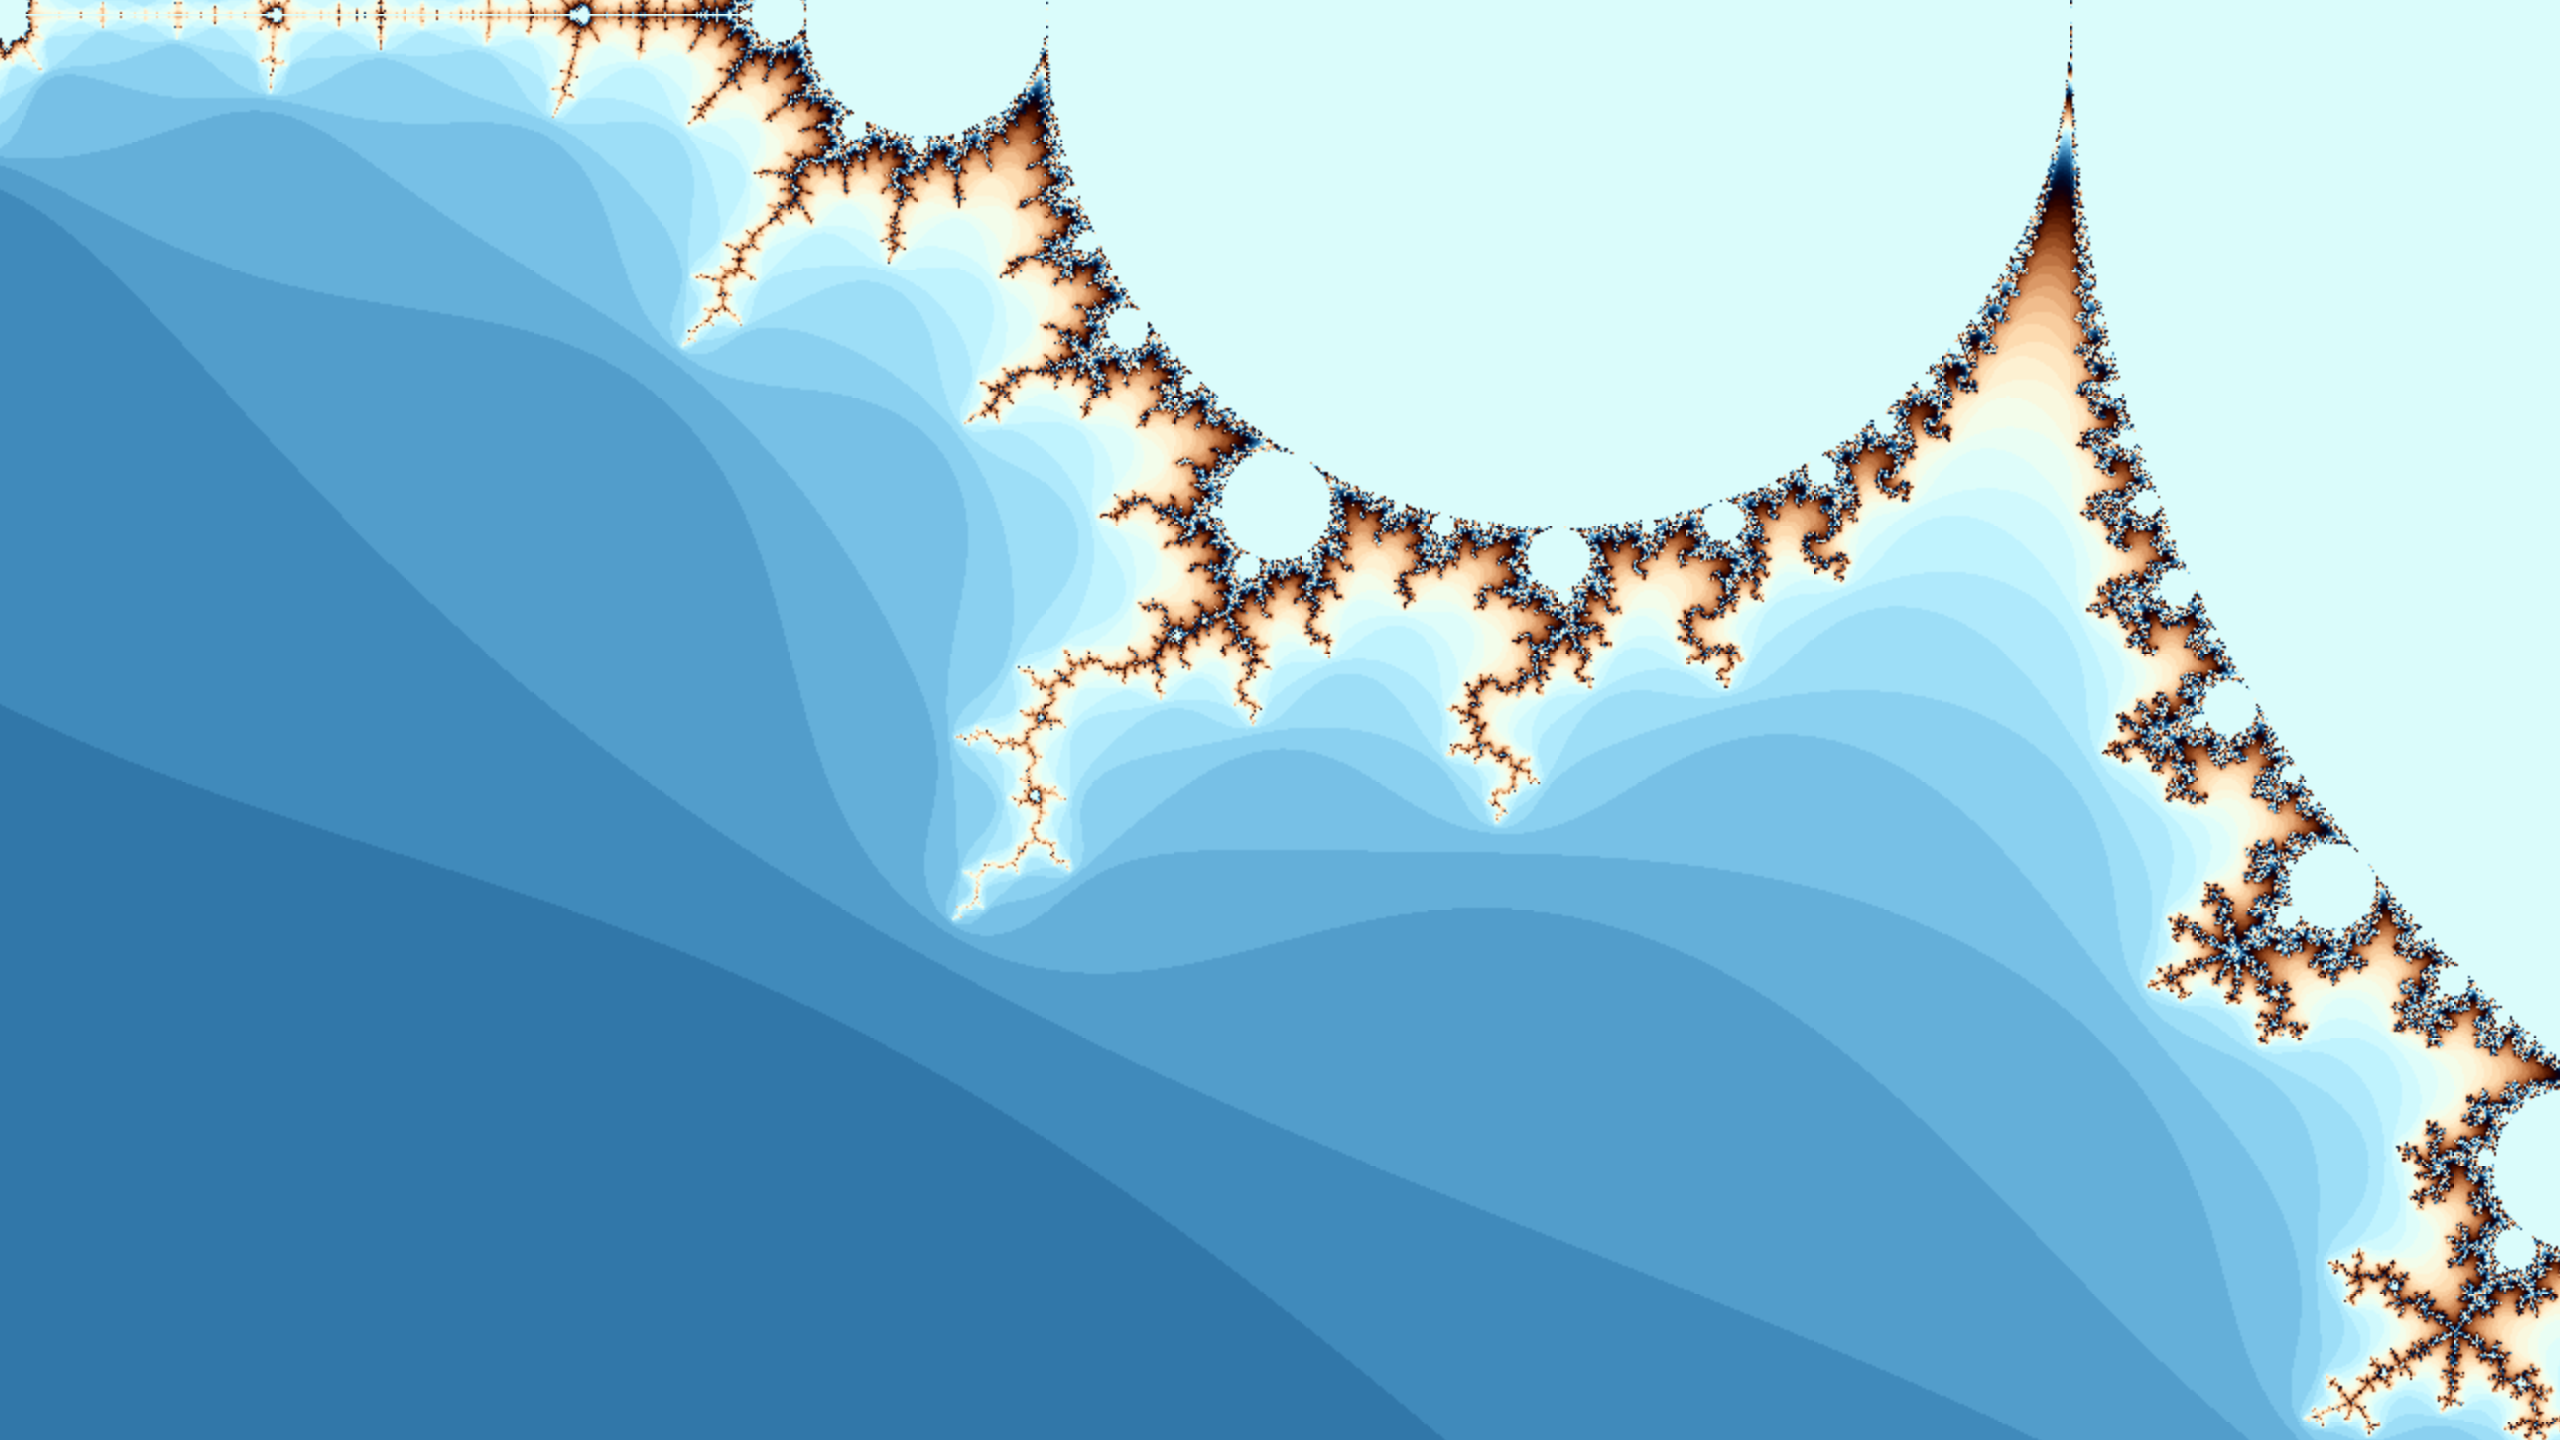
\includegraphics[width=0.2\textwidth]{img/Evaluation/border1} & 
\includegraphics[width=0.2\textwidth]{img/Evaluation/in1} \\
		\( (-1.38866,1.01930,2) \)                                 & \( (-1.13528, -0.34512, 2) \)                                 & \( (-0.21118, 0.07617, 3) \)                              \\
		
\includegraphics[width=0.2\textwidth]{img/Evaluation/out2} & \includegraphics[width=0.2\textwidth]{img/Evaluation/border2} & 
\includegraphics[width=0.2\textwidth]{img/Evaluation/in2} \\
		\( (-0.86151,0.37891,11) \)                                & \( (-0.73341, 0.21651, 11) \)                                 & \( (-1.75620, 0.00049, 10) \)                             \\
		
\includegraphics[width=0.2\textwidth]{img/Evaluation/out3} & \includegraphics[width=0.2\textwidth]{img/Evaluation/border3} & 
\includegraphics[width=0.2\textwidth]{img/Evaluation/in3} \\
		\( (-0.76671,-0.16323,25) \)                               & \( (-0.04666,0.98511, 25) \)                                  & \( (-0.11136, -0.04529, 25) \)                            \\
	\end{tabular}
	\caption{Testregionen der Evaluierung. Jeder der Punkte \( z \in \mathbb{C} \) entspricht dem Mittelpunkt der Region im Format \( (Re(z), Im(z), zoom) \) }
	\label{fig:testRegions}
\end{figure}

Die in den folgenden Abschnitten ausgewerteten Rechenzeiten für die Komponenten des Back- und
Frontends wurden in den entsprechenden Teilanwendungen in \( \mu s \) unter Verwendung der jeweiligen
Systembibliotheken (\verb|std::chrono|\footnote{\url{https://en.cppreference.com/w/cpp/chrono}} in \verb|C++| und \verb|Performance API|\footnote{\url{https://developer.mozilla.org/en-US/docs/Web/API/Performance}} in \verb|node.js|) gemessen.
Dabei stellt das so modifizierte Backend eine Erweiterung dar,
welche die gemessenen Zeiten zusätzlich in der Antwort der Regionsdaten an das Frontend
versendet. Dort werden diese aggregiert, mit den Zeiten des Frontend verknüpft und ausgegeben.

Um die Performance der folgenden Algorithmen auf der Mandelbrotmenge zu evaluieren,
müssen Regionen einzeln ausgewählt und die Performanz ihrer Berechnung verglichen werden.
Dafür haben wir die Mandelbrotmenge in drei Klassen unterteilt: Regionen in, am Rand und außerhalb
der Menge. Diese Aufteilung ist so gewählt, dass sich die Anzahl Iterationen pro Punkt innerhalb einer Klasse ähneln.
Dazu haben wir ebenfalls für jede der Klassen eine niedrige, mittlere und hohe Zoomstufe gewählt (siehe \autoref{fig:testRegions}).

Gemessen wurden alle folgenden Daten auf dem \verb|HimMUC|\footnote{\url{http://www.caps.in.tum.de/himmuc/}}
Cluster unabhängiger Rechenknoten des Lehrstuhls für Rechnerarchitektur und Parallele Systeme\footnote{\url{https://www.caps.in.tum.de/startseite/}} der TUM.
Dieses besteht aus jeweils 40 Raspberry Pi B\footnote{\url{https://www.raspberrypi.org/products/raspberry-pi-3-model-b/}} und
40 ODroids C2\footnote{\url{https://www.hardkernel.com/shop/odroid-c2/}}. Wobei ausschließlich die ODroid C2 Rechner verwendet wurden.
Auf dem Rechencluster wird als MPI-Implementierung \verb|OpenMPI|\footnote{\url{https://www.open-mpi.org/doc/v3.1/}} verwendet,
welches einen starken Fokus auf Effizienz legt und auch die Nutzung von Threads unterstützt, 
was laut der offiziellen \verb|MPI-Dokumentation|\footnote{\url{https://www.mpi-forum.org/docs/mpi-3.1/mpi31-report.pdf}} ein optionales Feature ist.

% Evtl. Namen der Paragraphen anpassen.
\subsection{MPI-Kommunikation}

\paragraph{Skalierung der MPI-Kommunikation}
Die Entwicklung der MPI-Kommunikationszeit bei steigender Anzahl an Workern ist wichtig für Annahmen folgender Evaluierungen und 
könnte Schwachstellen des Kommunikationskonzepts aufdecken.

In \autoref{fig:scaling_mpi} wird für jeden Regionstyp (Außen-, Rand-, Innenregion) die durchschnittliche MPI-Kommunikationszeit 
pro Anzahl an Workern dargestellt. Dabei wurde die Strategie mit Vorhersage (rekursiv) verwendet, 
so dass die Worker eine möglichst identische Rechenzeit haben, womit die MPI-Kommunikation aller Worker 
auf den etwa gleichen Zeitpunkt fällt, was den Worst-Case darstellt. 
Eine anderweitige Parallelisierung mittels OpenMP oder SIMD wurde nicht vorgenommen.
%Implementierung noch erwähnen?
\begin{figure}[h!]
	\centering
	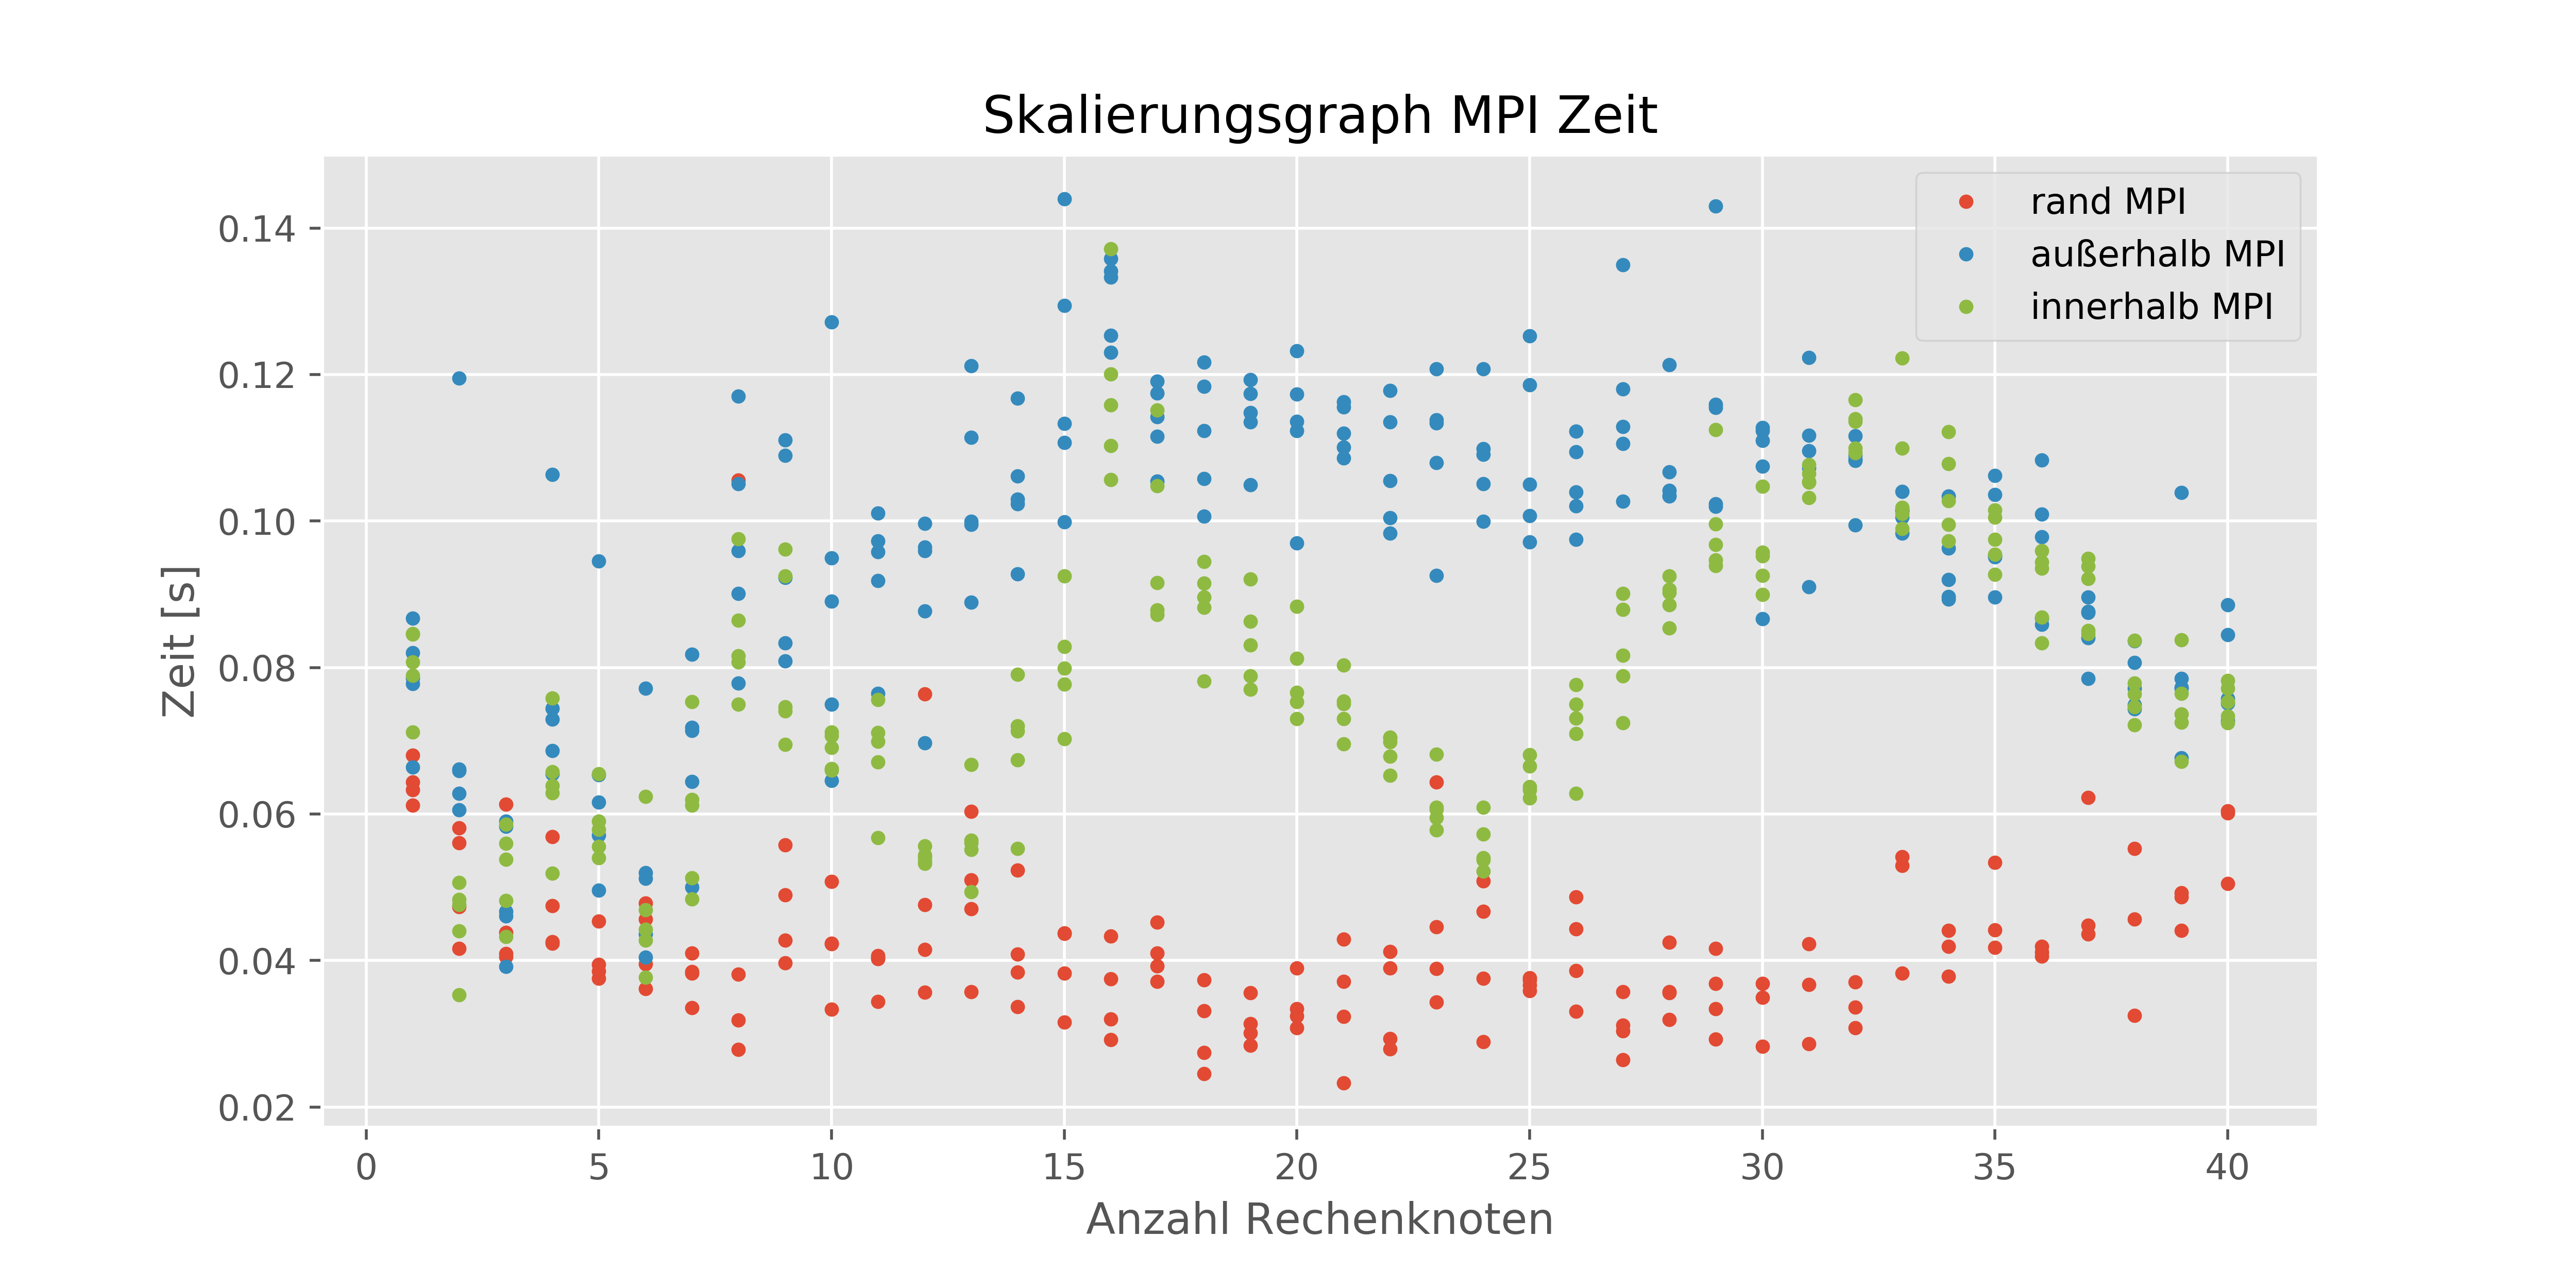
\includegraphics[width=0.9\linewidth]{img/Evaluation/scaling_mpi.png}
	\caption{Skalierung der MPI-Kommunikation. Strategie mit Vorhersage (rekursiv). Ohne OpenMP oder SIMD.}
	\label{fig:scaling_mpi}
\end{figure}
Es ist zu erkennen, dass die MPI-Kommunikationszeit für alle Regionstypen annähernd konstant, wenn verglichen mit der Rechenzeit bleibt.
Dabei verhalten sich


für Außenregionen (blau) zunächst ansteigt und dann auf einem konstanten Niveau bleibt.
Dies ist der Fall, da alle Teilregionen sehr ähnlich sind und eine extrem kurze Rechenzeit haben, wodurch alle Worker etwa zur selben Zeit ihre Berechnung abschließen und die Ergebnisse senden. 
Damit kommen die Rechenergebnisse zur selben Zeit im Host an, 
welcher die Empfangsoperationen aber nur sequenziell und nicht parallel ausführt. 
Das verursacht eine Aufstauung der Nachrichten, was in einer maßgeblichen Verlangsamung der MPI-Kommunikation resultiert.
% Der Graph bleibt konstant, weil die Nachrichtenlänge sinkt und damit das Empfangen und das anschließende kopieren kürzer ausfällt.

Für Randregionen (rot) fällt auf, dass die MPI-Kommunikationszeit konstant bei etwa \( 40 \) Millisekunden liegt.
Für diesen Regionstyp liefert der Balancer wenige Teilregionen mit exakt gleicher Rechenzeit (siehe \hyperref[sec:lastbalancierung_eval]{Evaluierung der Lastbalancierung}), 
was das für die Außenregionen angesprochene Problem abwendet. 
Die Rechenergebnisse werden nicht gleichzeitig gesendet bzw. empfangen, was einen Stau im Host verhindert.

Für Innenregionen (grün) ist eine deutliche Fluktuation der Kommunikationszeit zu erkennen.
Es fällt auf, dass die Kommunikationszeit ein deutliches Maximum bei \( 16 \) bzw. \( 32 \) und ein Minimum bei \( 24 \) Workern erreicht.
Das liegt daran, dass die Lastbalancierung besser wird, je näher die Workeranzahl einer Zweierpotenz ist.
Wie bei den Außenregionen führen ähnliche Rechenzeiten zur Anstauung von Nachrichten im Host, was die MPI-Zeit erhöht.
Dieses Verhalten der lokalen Extrema zeigt sich in der gesamten Kurve der Innenregionen.

Eine Verbesserung der MPI-Kommunikation wird als nicht nötig erachtet, da für den Nutzer die Randregionen am interessantesten sind und das Problem des Flaschenhalses im Host hierbei keine Rolle spielt.

\paragraph{Speedup-Faktor durch Parallelisierung mittels MPI}

Eine wichtige Performancemetrik ist, wie sich die Rechenzeit der einzelnen Teilregionen im Vergleich zur Anzahl der an der Berechnung beteiligten Worker verhält.

In \autoref{fig:scaleGraph} ist für jeden Regionstyp (Außen-, Rand-, Innenregion) ein Skalierungsgraph abgebildet, 
der den Speedup-Faktor in Abhängigkeit der Anzahl der genutzten Worker darstellt. 
Dabei kam weder OpenMP noch SIMD zum Einsatz. Es wird erwartet, dass sich der Speedup-Faktor \( s \) ungefähr nach \( s \approx \frac{c_1 + c_2}{(c_1/n) + c_2} \) verhält, 
wobei \( n \) die Anzahl der an der Berechnung beteiligten Worker, 
\( c_1 \) die Rechenzeit ohne jegliche Parallelisierung (also mit genau einem Worker) und \( c_2 \) der konstante MPI-Kommunikationsoverhead ist. 
Da für jeden Regionstyp die \( c_1 \) unterschiedlich groß ist, fällt \( c_2 \) mehr oder weniger ins Gewicht, 
was zu unterschiedlichen Speedup-Faktoren führt. 
Konkret wird erwartet, dass für die Speedup-Faktoren die Relation Außenregion \( \leqslant \) Randregion \( \leqslant \) Innenregion gilt.

\begin{figure}[h!]
	\centering
	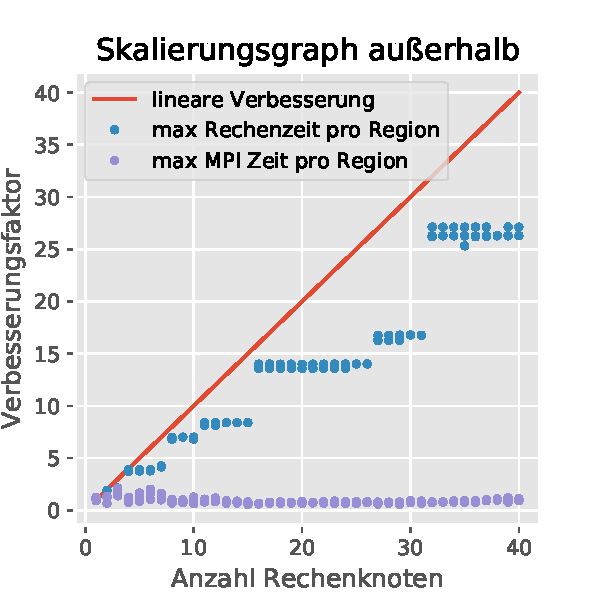
\includegraphics[width=0.32\linewidth]{img/Evaluation/scale_graph_outside}
	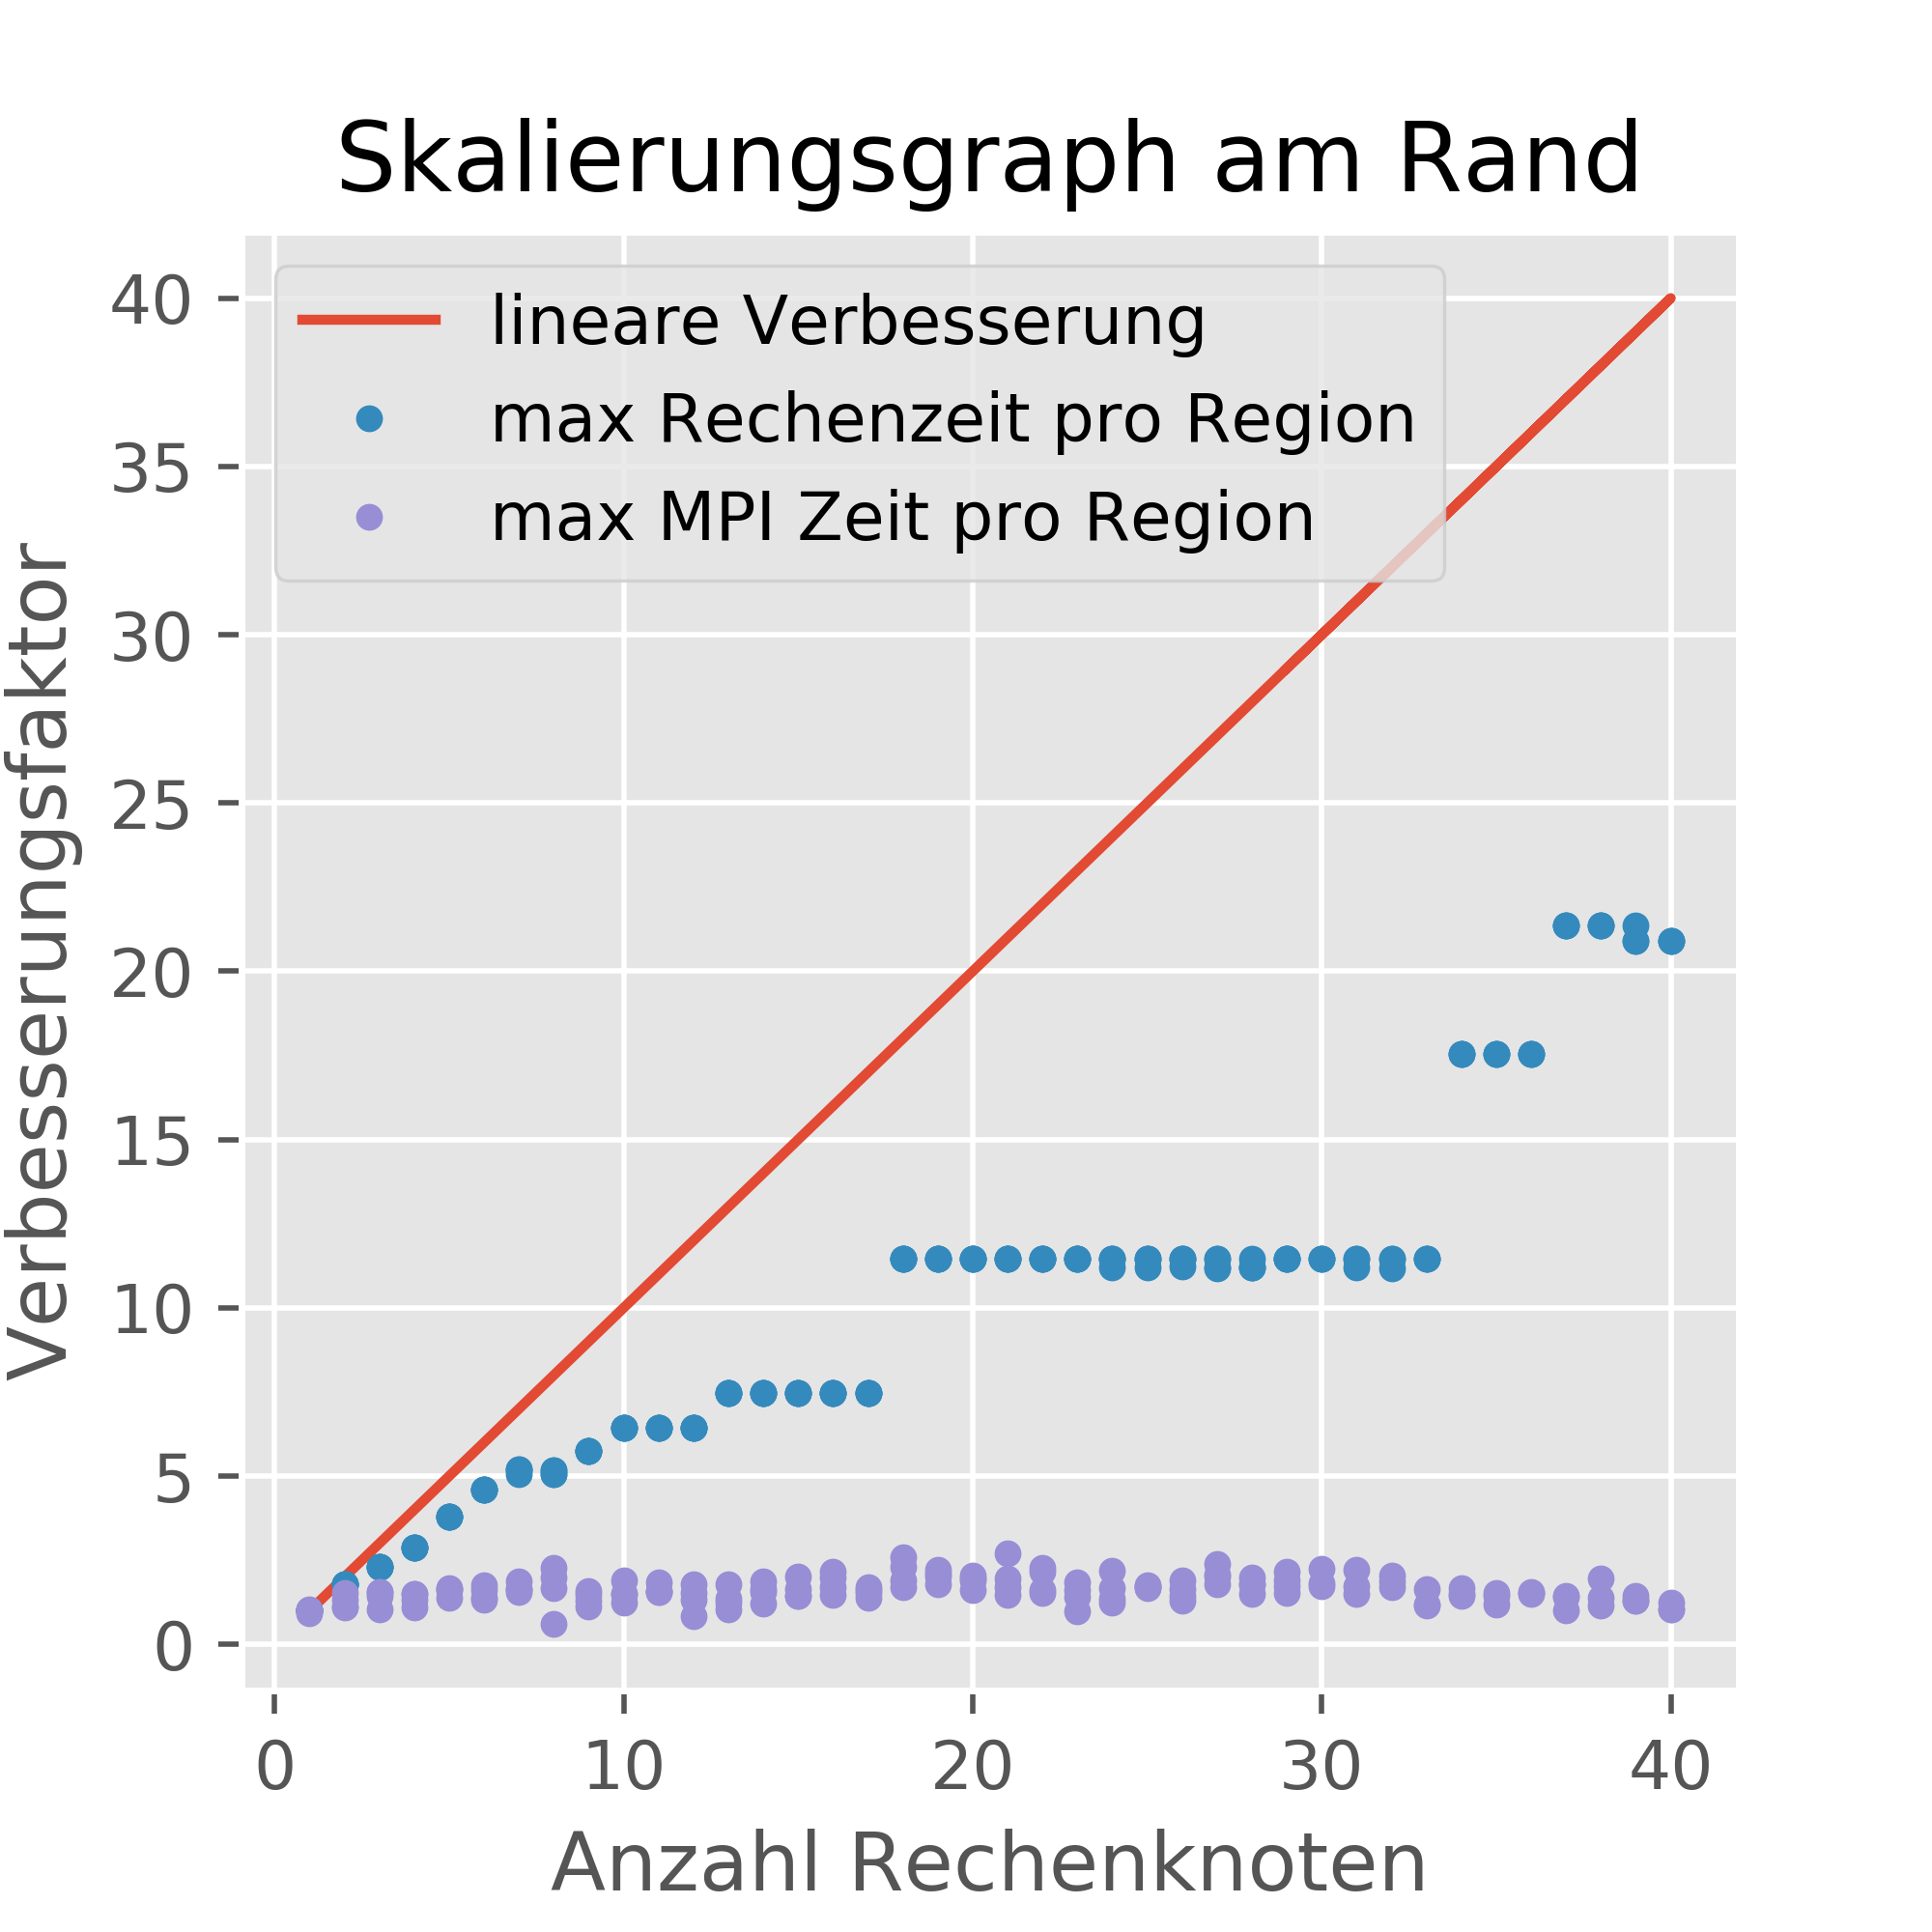
\includegraphics[width=0.32\linewidth]{img/Evaluation/scale_graph_border}
	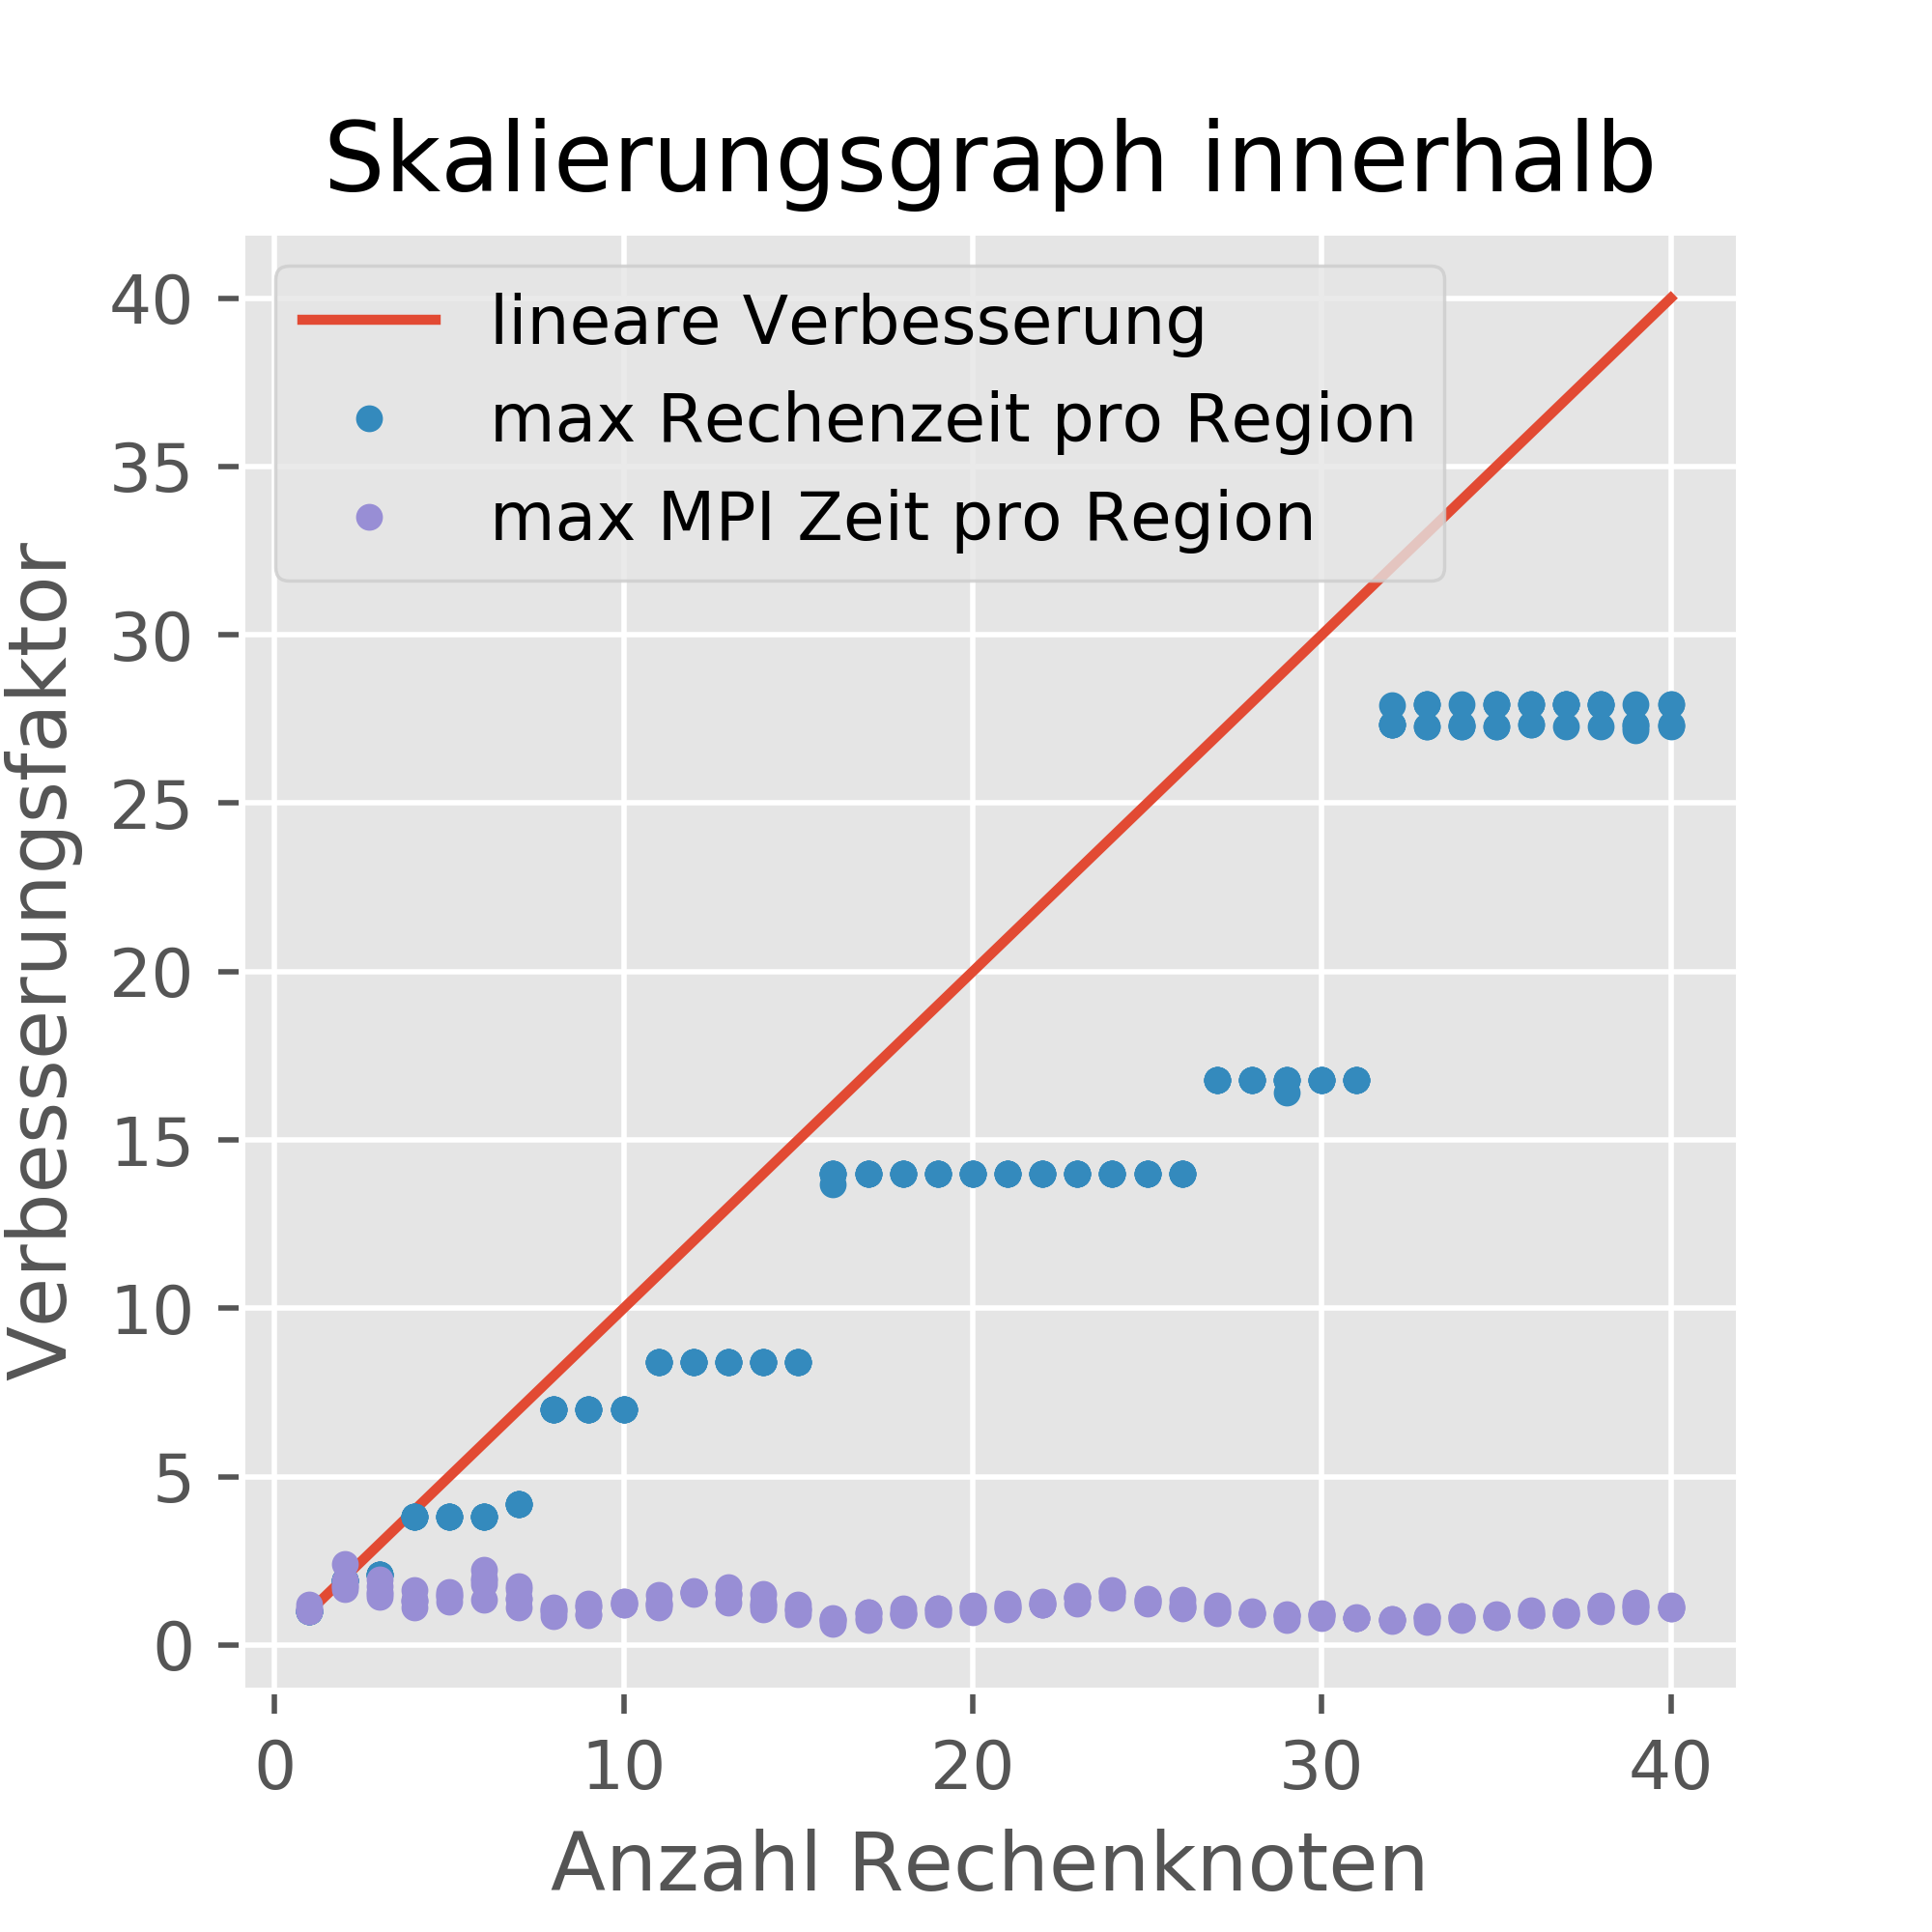
\includegraphics[width=0.32\linewidth]{img/Evaluation/scale_graph_inside}
	\caption{Speedup-Faktor von \( 1-40 \) Rechenknoten. Strategie mit Vorhersage (rekursiv). Ohne OpenMP oder SIMD}
	\label{fig:scaleGraph}
\end{figure}
\begin{figure}[h!]
	\centering
	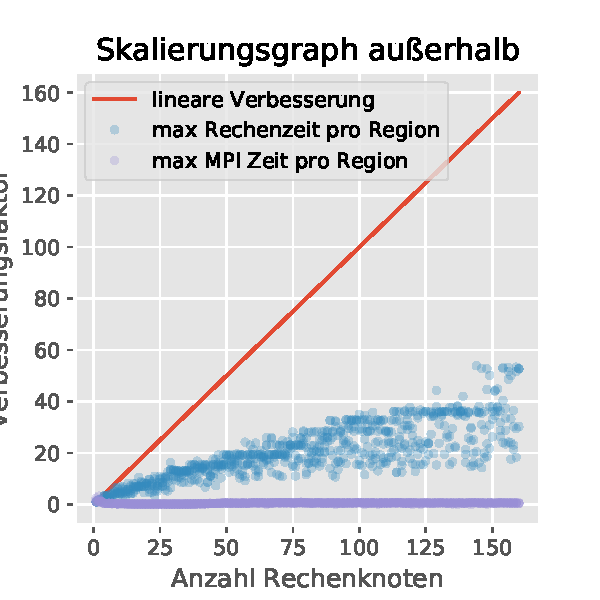
\includegraphics[width=0.32\linewidth]{img/Evaluation/scale_graph_outside_more_nodes}
	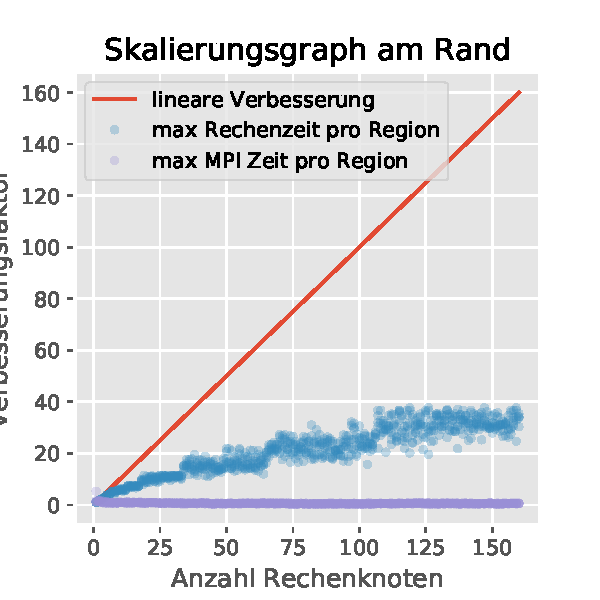
\includegraphics[width=0.32\linewidth]{img/Evaluation/scale_graph_border_more_nodes}
	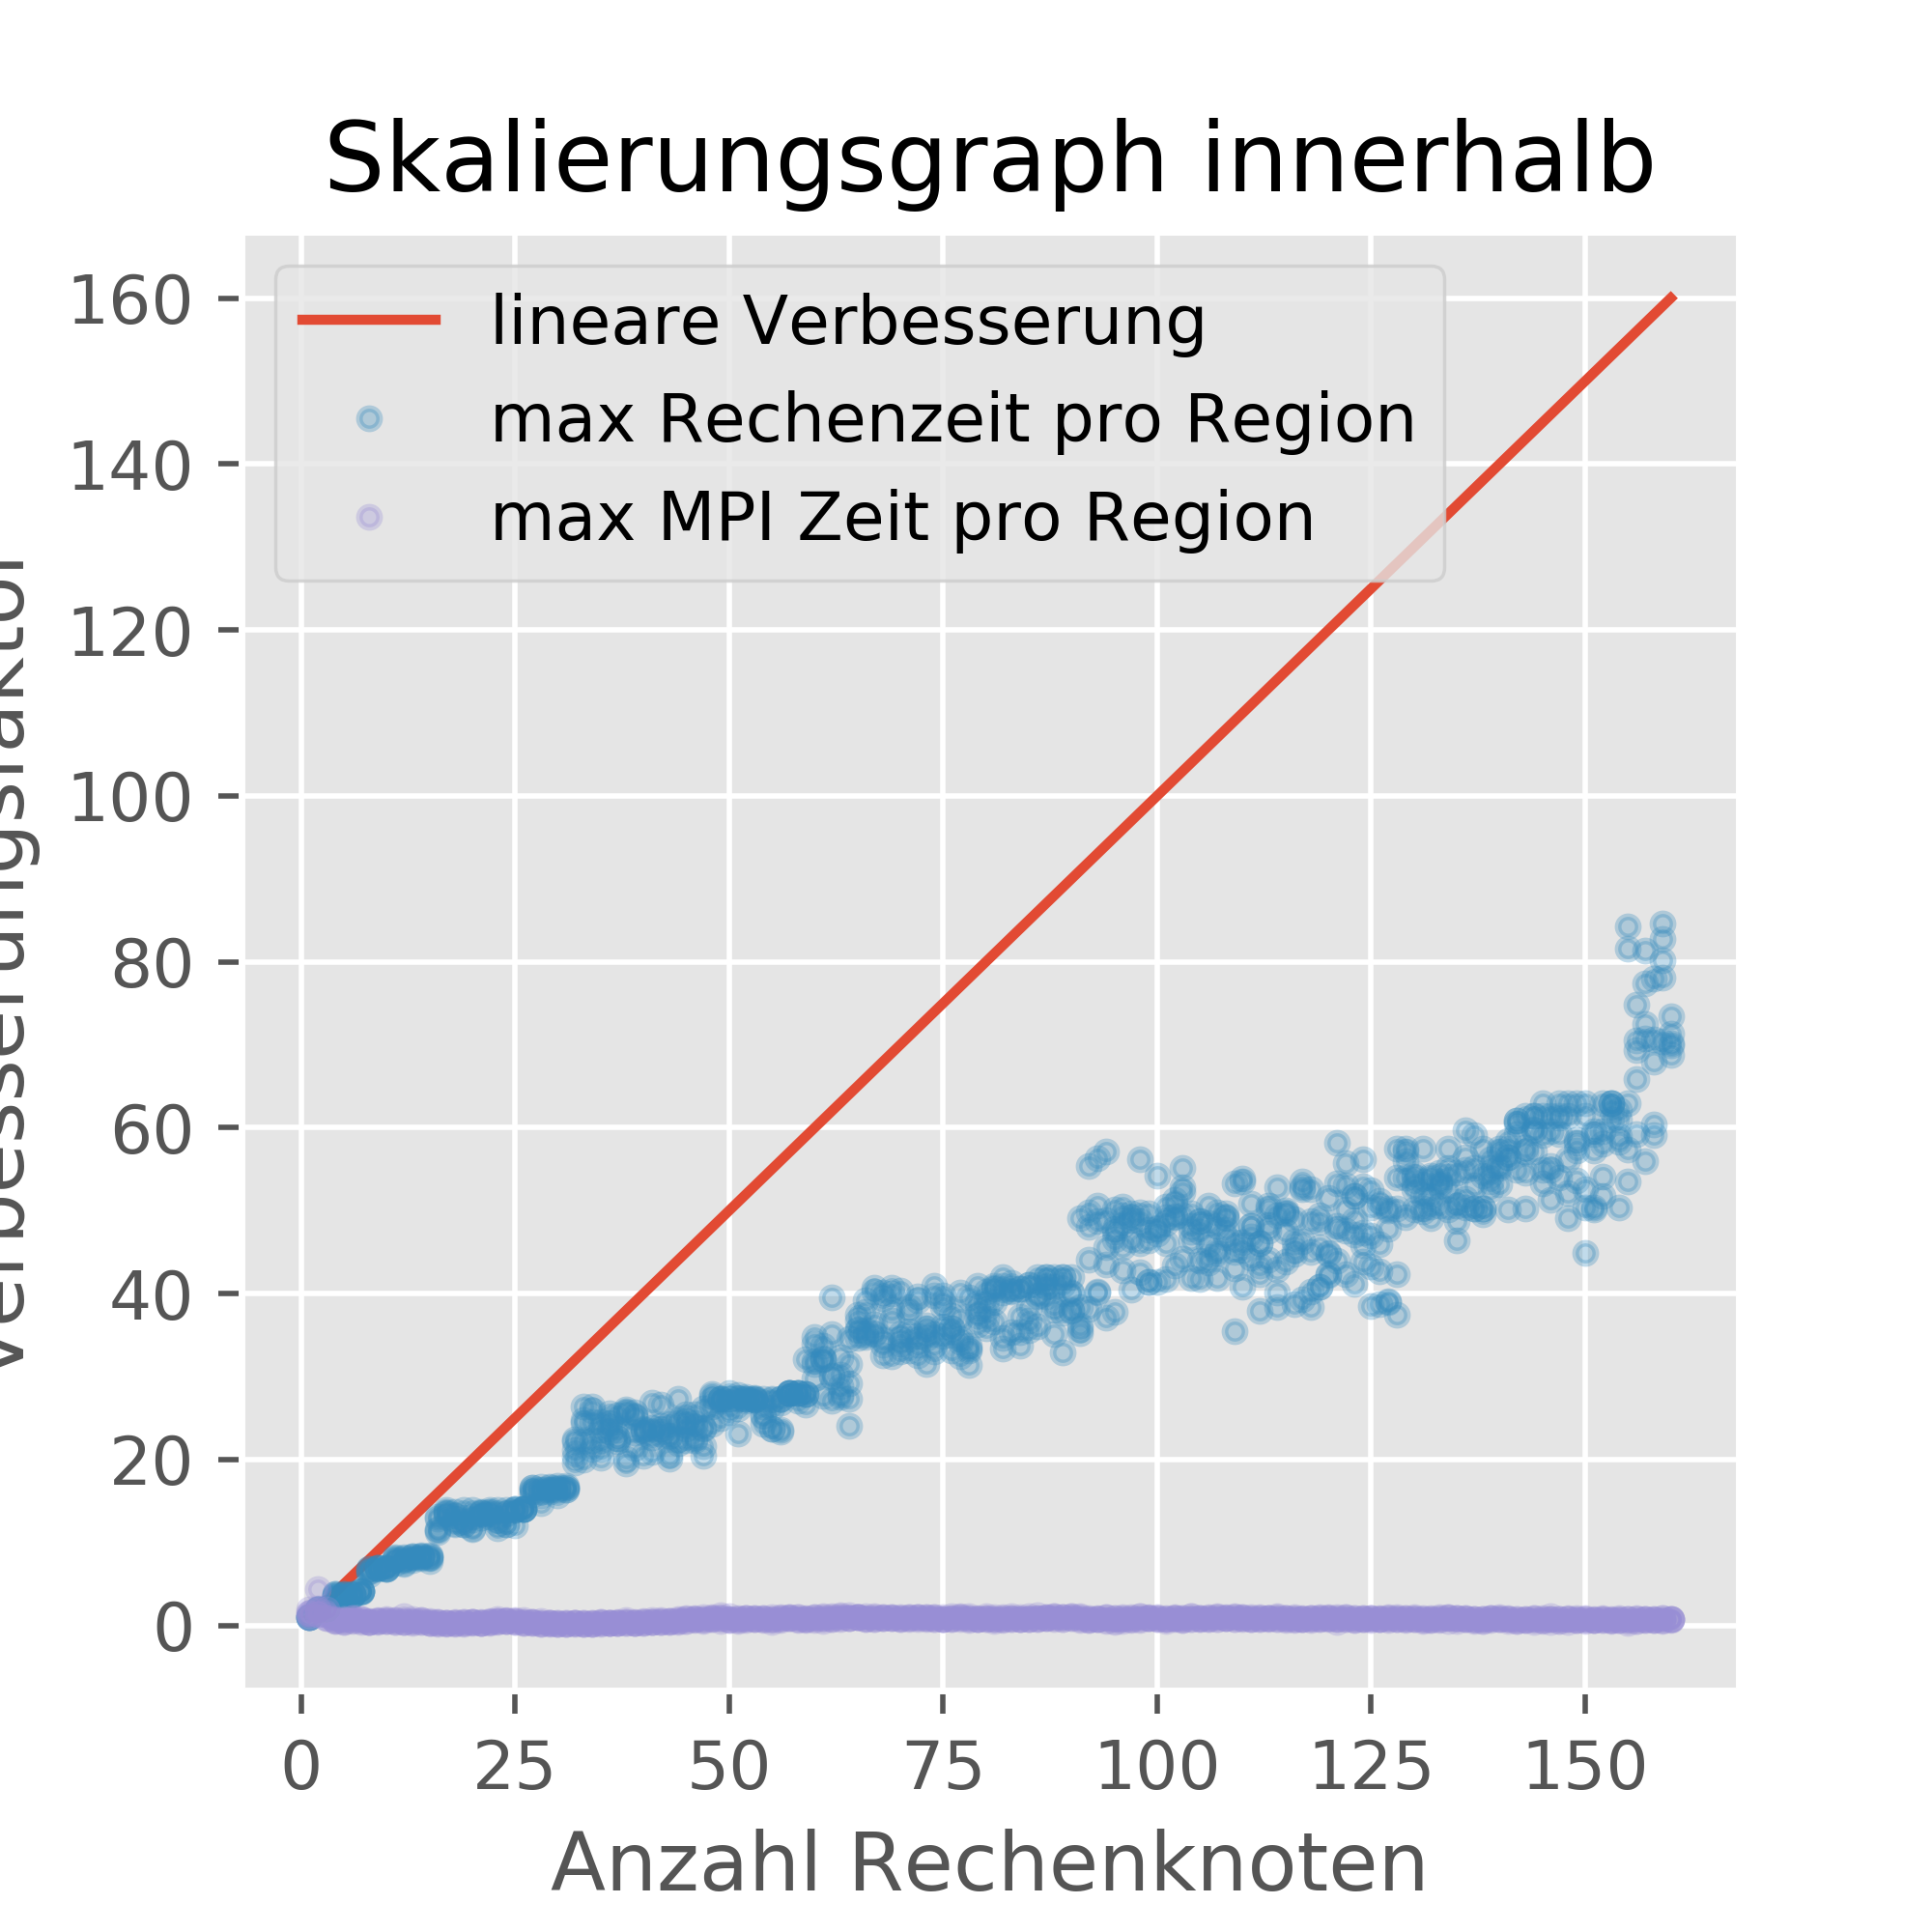
\includegraphics[width=0.32\linewidth]{img/Evaluation/scale_graph_inside_more_nodes}
	\caption{Speedup-Faktor von \( 1-160 \) MPI-Prozessen, dabei erhält jeder Knoten 4 MPI-Prozesse. Strategie mit Vorhersage (rekursiv). Ohne OpenMP oder SIMD}
	\label{fig:scaleGraphMoreNodes}
\end{figure}

Es ist in \autoref{fig:scaleGraph} zu erkennen, dass der Speedup-Faktor bei 40 Workern für Außenregionen bei 27, für Randregionen bei 22 und für Innenregionen bei 27 liegt. Auch für 160 Workern ist in \autoref{fig:scaleGraphMoreNodes} ein Speedup von 40 für Außen- und Randregionen bzw. 65 für Innenregionen zu erkennen. Hierbei flacht der Speedup-Faktor aber schon erkennbar ab, was für eine Annäherung an sein Maximum \( s_{max} \approx \frac{c_1 + c_2}{c_2} \) spricht.
Damit stimmen die Messergebnisse mit den Erwartungen überein.


% OpenMP & MPI skalierung
% Bar graph (1 MPI Prozess pro worker, 1 MPI Prozess & 4 OpenMP pro Worker, 4 MPI Prozesse pro worker)
% 	Worker & Iteration Anzahl fest, optimal wählen, Randregion
\subsection{OpenMP}
In den vorangegangenen Evaluierungen wurde nur ein Rechenkern pro Computer im Cluster für die Berechnung der Mandelbrotmenge genutzt. 
Nun soll die Performancesteigerung durch die Nutzung von mehreren Rechenkernen pro Computer 
untersucht werden. Bei dem für diese Evaluierung verwendeten ODroid C2 stehen vier Rechenkerne zur Verfügung.
In \autoref{fig:parallelism} ist durchschnittliche Rechenzeit von einem MPI-Prozess (rot), zwei MPI-Prozessen (blau), einem MPI-Prozess 
mit 4 OpenMP-Threads (lila) und vier MPI-Prozessen (grün) pro ODroid dargestellt. 
Es wird erwartet, dass sich die Speedup-Faktor \( s \) nach \( s \approx \frac{c}{n} \) verhält, 
wobei c die Rechenzeit des einen MPI-Prozesses (rot) und n die Anzahl an verwendeten Prozessen bzw. 
Threads pro ODroid darstellt.
\begin{figure}[h!]
	\centering
	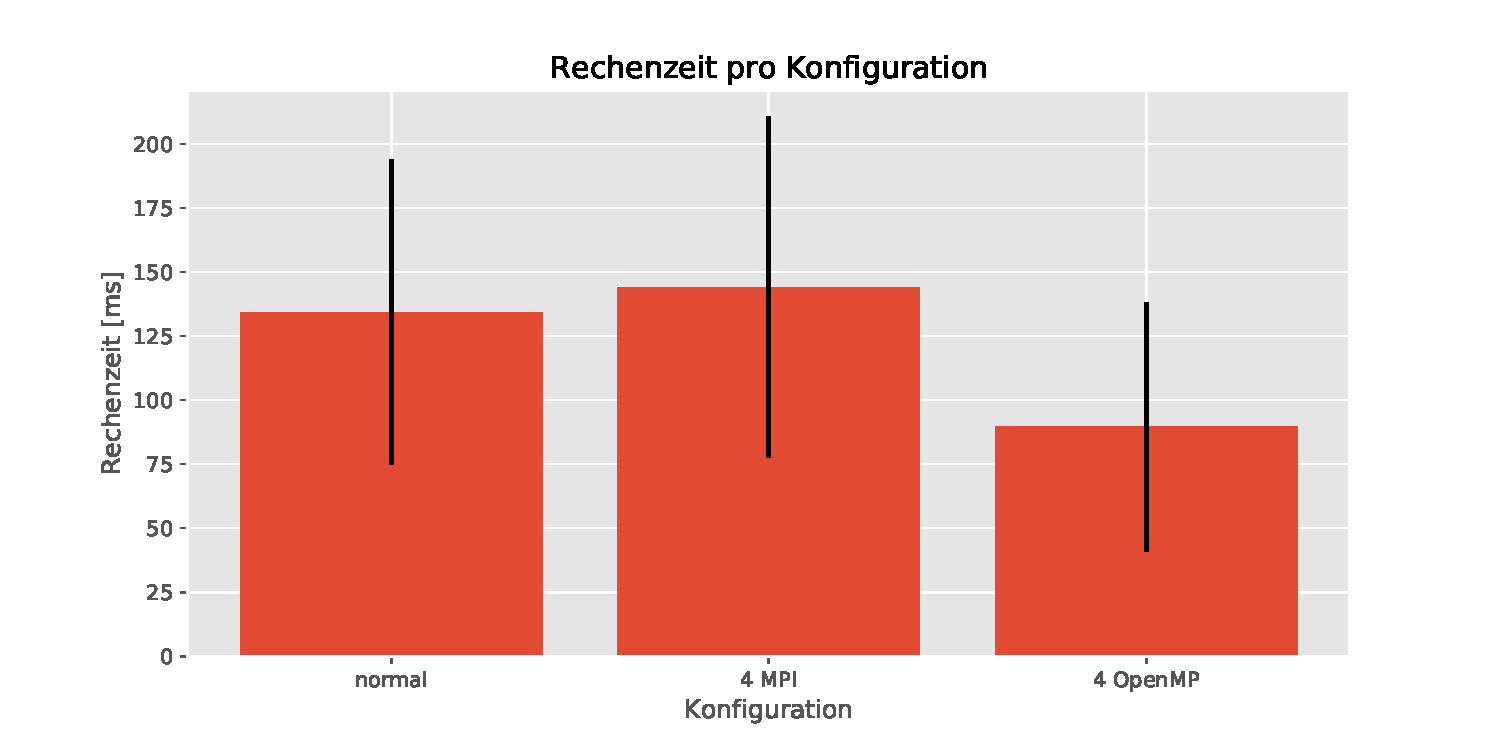
\includegraphics[width=0.9\linewidth]{img/Evaluation/parallelism.pdf}
	\caption{Rechenzeiten mit verschiedenen Parallelisierungen. Strategie mit Vorhersage (rekursiv). Ohne SIMD.}
	\label{fig:parallelism}
\end{figure}

Für einen MPI-Prozess mit vier OpenMP-Threads pro ODroid wurde ein Speedup-Faktor von 3,2 und für vier MPI-Prozesse 
pro ODroid wurde ein Speedup von ca. 3,9 gemessen. 
OpenMP bleibt damit etwas hinter den Erwartungen zurück. 
Dies ist der Fall, da für die OpenMP-Threads keine Lastbalancierung durch den Balancer durchgeführt werden kann. 
Stattdessen weißt OpenMP jedem Thread ein Pixel der Mandelbrotmenge zur Berechnung zu. 
Ist die Berechung abgeschlossen bekommt der Thread einen neuen Pixel zugewiesen. 
Der durch dieses dynamische Scheduling entstehende Overhead sorgt für den Performanceverlust. 
Die vier MPI-Prozesse hingegen müssen die ihnen zugewiesenen Teilregionen nicht mehr aufteilen, 
da dies der Lastbalancierer bereits erledigt hat.


\subsection{SIMD}

% Niels:
% PLOTS: (mandelbrot 32, 64, simd 32,  64, 80 bit default)
% comp time vs iteration count plot
% speed up factor vs number of iterations
% (niedriger, höher ist besser)


% refactor:
% three bar graphs - average computation time for worst 25%, average 50% and best 50%
% one figure showing where SIMD achieves best increase in performance (see notebook)

SIMD unterstützt in den Präzisionen 32 und 64 bit Parallelisierung von einer Rechenoperationen auf
4 beziehungsweise 2 unterschiedlichen Werten. Der Effekt beläuft sich dabei, wie in \autoref{fig:SIMD-speedup} zu sehen,
bei einer Beschränkung auf 1019 Iterationen auf eine durchschnittliche Beschleunigung um den Faktor $\approx2,3$ und $\approx1,2$.

\begin{figure}
	\centering
	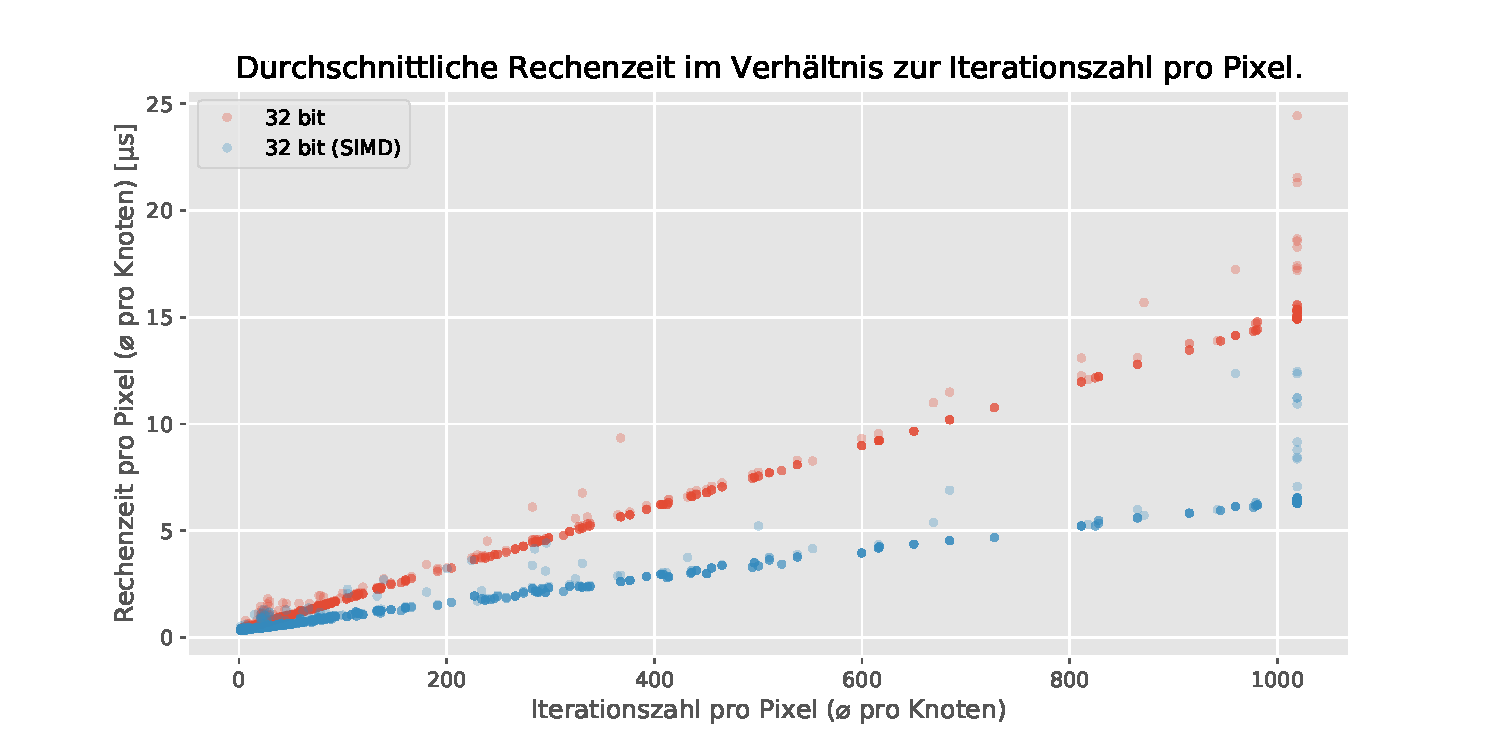
\includegraphics[height=3.5cm]{img/Evaluation/simd/itvscmp32.pdf}
	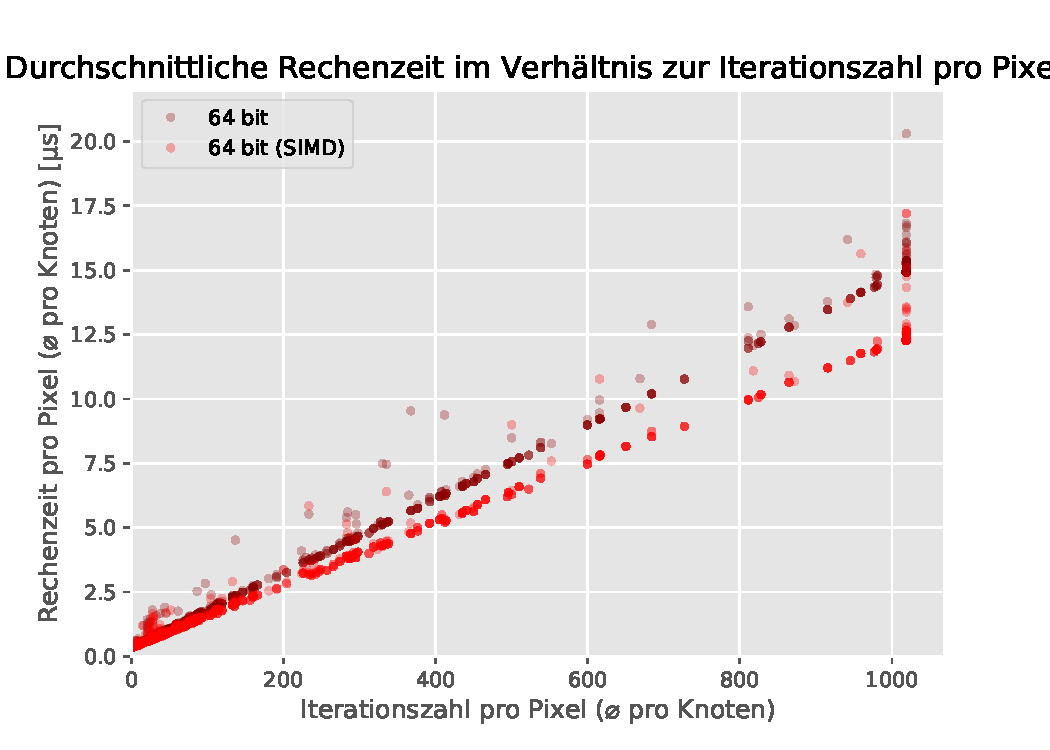
\includegraphics[height=3.5cm]{img/Evaluation/simd/itvscmp64.pdf}
	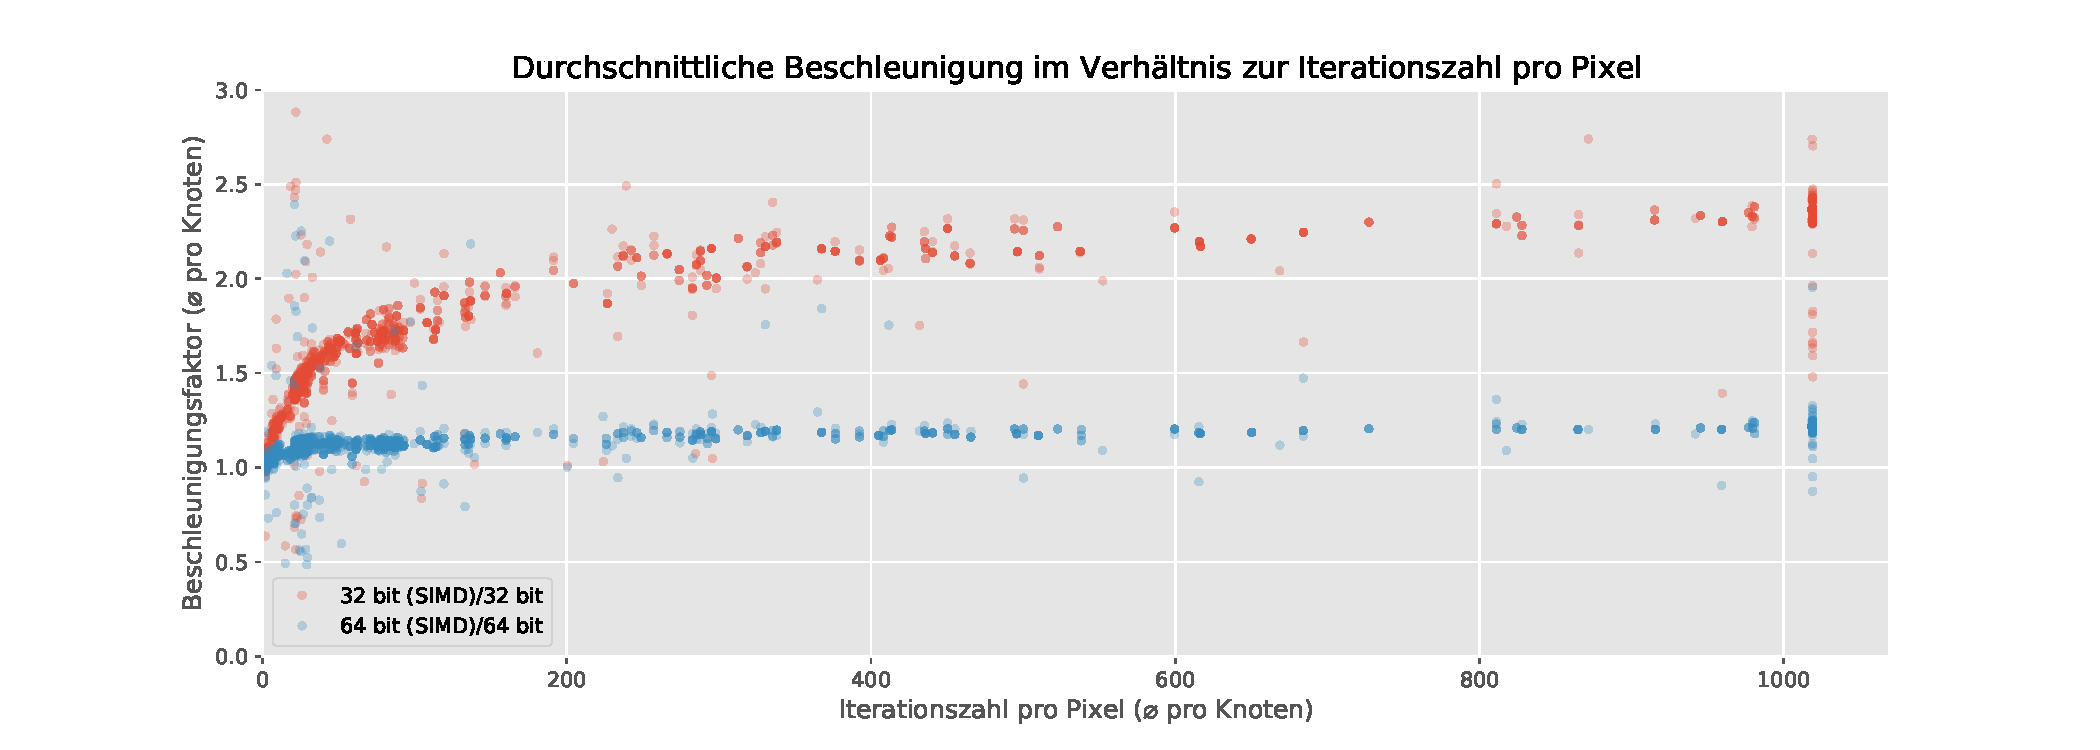
\includegraphics[height=5cm]{img/Evaluation/simd/speedup.pdf}
	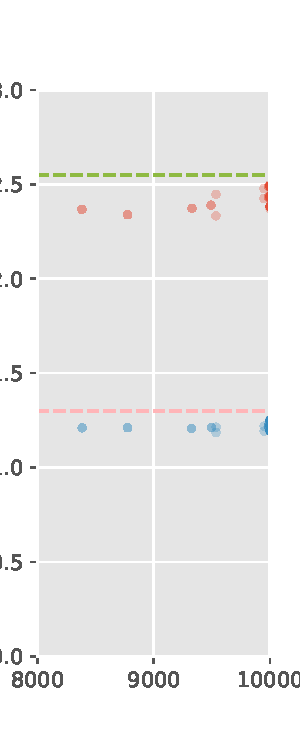
\includegraphics[height=5cm]{img/Evaluation/simd/speedup_10000_crop.pdf}
	\caption{Vergleich der Performanzen der Implementierungen mit und ohne SIMD bei bis zu 1019 Iterationen über 360 Regionen in 10 Wiederholungen.}
	\label{fig:SIMD-speedup}
	\label{fig:SIMD-speedup-vs-comptime}
\end{figure}

Dass die Performanzerhöhung nicht genau $4$ oder $2$ ist, lässt sich mit dem erhöhten Aufwand der Verwendung
der SIMD Instruktionen erklären.
Da hierzu die Werte aus den normalen Registern in spezielle SIMD-Register und zurück
kopiert werden müssen, entsteht eine gewisse Verzögerung durch zusätzliche Transportoperationen.
Die tatsächliche Rechenzeit für eine Vektorisierung von \(n\) Punkten sollte also \(t_{SIMD} \approx \frac{t_{normal}}{n}+ const\) entsprechen.

Je größer die benötigte Zahl an Operationen, desto weniger fällt dieser konstante Zusatzaufwand ins Gewicht.
Dies kann zum Beispiel in \autoref{fig:SIMD-speedup-vs-comptime} beobachtet werden.
Steigert man die maximale Iterationszahl von 1019 auf bis zu 10000 steigt dieser Speed-Up nicht wesentlich weiter.
Der Speedup entwickelt sich dann asymptotisch gegen $2.55$ und $1.3$. Details zu dieser Entwicklung sind in \autoref{par:SIMD-speedup-entwicklung} zu finden.

Zudem werden für eine Menge an Punkten stets die Zahl an Iterationen durchgeführt,
die das Maximum aller Iterationszahlen der Punkte ist.
Bei Iterationszahlen \(i_k\) des Punktvektors \(p\) ist daher
anstatt einer Rechenzeit von \(\sum_{k \in p} \frac{i_k }{ | p | }\) eine Rechenzeit von
\(\sum_{k \in p} \frac{max(i_k)_{k \in p }}{|p|} = max(i_k)_{k \in p }\) pro Punktvektor zu erwarten.
Damit wird die Beschleunigung durch SIMD kleiner, je inhomogener die Iterationszahlen sind.
Dass die Iterationszahlen im Allgemeinen am Rand der Mandelbrotmenge inhomogener sind,
wo auch die Gesamtrechenzeit geringer ist, sollte bei der Betrachtung von \autoref{fig:SIMD-speedup-vs-comptime} berücksichtigt werden.

%\begin{figure}
%	\centering
%	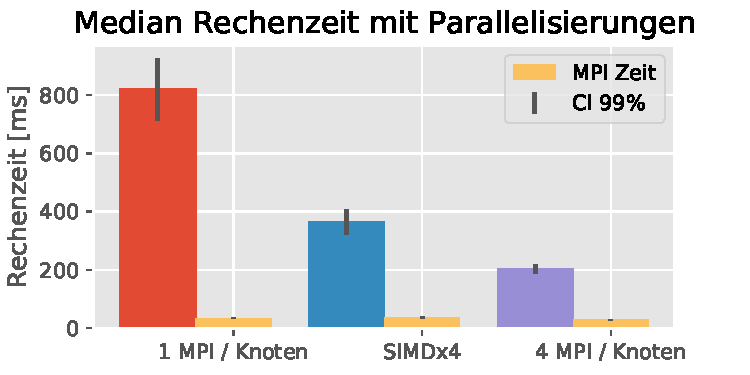
\includegraphics[width=0.45\linewidth]{img/Evaluation/simd/parallelismNaiveBalancing.pdf}
%	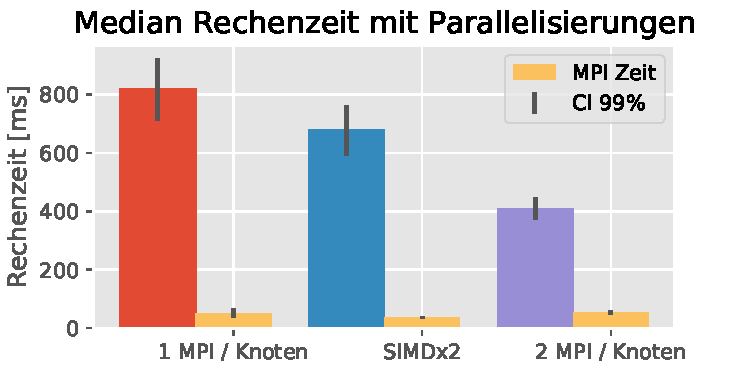
\includegraphics[width=0.45\linewidth]{img/Evaluation/simd/parallelismNaiveBalancing64.pdf}
%	\caption{Vergleich zwischen der Performanz mit mehr MPI-Prozessen und SIMD bei naiver Lastbalancierung.
%		Eine Erhöhung der Anzahl an Rechenknoten führt zu einer deutlich größeren Beschleunigung.}
%	\label{fig:SIMDvs4timeMore}
%\end{figure}

Insgesamt kann mit SIMD eine deutliche Beschleunigung des Systems bewirkt werden.
%Stehen jedoch mehr Rechenkerne zur Verfügung, schneidet wie in \autoref{fig:SIMDvs4timeMore} zu sehen eine Erhöhung der MPI-Prozesse besser ab.
Da die Parallelisierungsmethode zu MPI und OpenMP unabhängig ist, führt die Anwendung von SIMD generell
zu einer Erhöhung der Performanz und empfiehlt sich bei einfacher Umsetzbarkeit.

\subsection{Lastbalancierung}\label{sec:lastbalancierung_eval}
% Florian
% Wir haben zwei Klassen (naive, prediction) und wählen davon jeweils den besten 
% (naive Recursive, prediction Recursive)
Zur Lastbalancierung gibt es zwei Strategien in jeweils zwei Varianten, zur Evaluierung wird allerdings nur die rekursive Variante der beiden Strategien betrachtet.
Man stellt leicht fest, dass die nicht-rekursive Variante für Primzahlen als Worker-Anzahl schlecht ist, weil dabei nur eine Aufteilung in Zeilen oder Spalten möglich ist.
Da die Aufteilungsmöglichkeiten zusätzlich durch die Betrachtung von Tiles als atomaren Einheiten beschränkt werden, erzeugt diese Variante bereits für eine geringe Anzahl an Workern verhältnismäßig viele Leerregionen (d.h. untätige Worker).
Deshalb wird für die Evaluation jeweils die rekursive Variante verwendet.

% Erst naiver Balancer, dann prediction dafür jeweils:
% 	Plot der distribution function (Median, Max)
% 	Maximale Rechenzeit & Wie gut sind die Werte um den Median verteilt
% 	3 Plots mit Regionen außerhalb, im Rand und innerhalb der Mandelbrotmenge
Um die naive Strategie und die Strategie mit Vorhersage zu vergleichen werden drei Klassen von Regionen betrachet (vgl. \autoref{fig:testRegions}), für die es unterschiedliche Erwartungen gibt:

\begin{itemize}
	\item innere Regionen: Die Rechenzeiten sind bei beiden Strategien gleichmäßig hoch
	\item äußere Regionen: Die Rechenzeiten sind bei beiden Strategien gleichmäßig niedrig
	\item Randregionen: Für die naive Strategie wird hier eine große Streuung der Rechenzeiten erwartet. Die Strategie mit Vorhersage sollte für eine Ballung um den Mittelwert sorgen.
\end{itemize}

Weiterhin wird erwartet, dass der Mittelwert der Rechenzeit pro Regionsklasse für die beiden Strategien gleichbleibt, da die selbe Region mit der selben Anzahl an Workern berechnet wird.
Für die Messungen hier wurden immer 17 Worker verwendet.

% Bilder und Stuff
% Vorhersage nie perfekt, deshalb Ausreißer nach oben/unten
% Teilweise größere/kleinere Teilregionen erstellt
In den folgenden Diagrammen wird die statistische Dichte der Rechenzeiten für die naive Strategie und die Strategie mit Vorhersage dargestellt.
Bei einer guten Lastbalancierung sollten sich die Rechenzeiten also um den Mittelwert ballen und die maximale Rechenzeit gering sein.

\begin{figure}
	\centering
	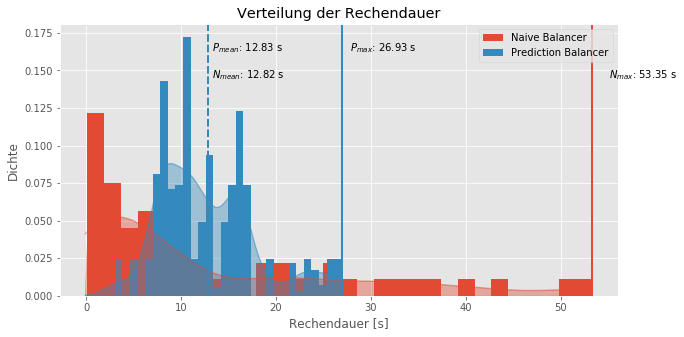
\includegraphics[width=0.9\linewidth]{img/Evaluation/balancers/balancers_border.png}
	\caption{Verteilung der Rechenzeiten für Randregionen}
	\label{fig:balancers_border}
\end{figure}

Den Unterschied zwischen naiver Strategie (rot) und Strategie mit Vorhersage (blau, leicht durchsichtig) sieht man besonders gut in der Verteilung für Randregionen (\autoref{fig:balancers_border}).
Die blauen Balken haben ihr Maximum in der Nähe des Mittelwerts, während die roten Balken viel mehr über den Wertebereich verteilt sind.
Dass die Strategie mit Vorhersage vom Mittelwert abweicht und auch einige Ausreißer nach oben und unten hat lässt sich auf Ungenauigkeiten in der Vorhersage zurückführen, welche am Rand der Mandelbrotmenge besonders ausgeprägt sind (vgl. \autoref{par:load_balancing_prediction}).

% TODO: Bilder in Breite und Höhe anpassen
\begin{figure}
	\centering
	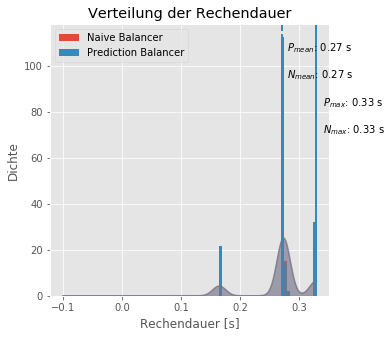
\includegraphics[width=0.45\linewidth]{img/Evaluation/balancers/balancers_outside_slim.png}
	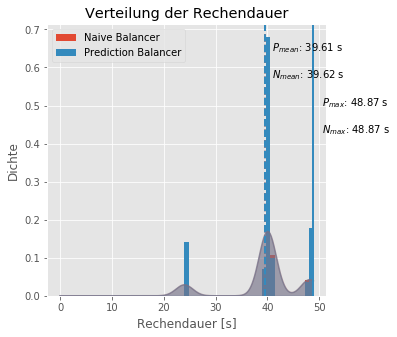
\includegraphics[width=0.45\linewidth]{img/Evaluation/balancers/balancers_inside_slim.png}
	\caption{Verteilung der Rechenzeiten für innere und äußere Regionen}
	\label{fig:balancers_inside_outside}
\end{figure}

Auch bei den inneren und äußeren Regionen wurde das erwartete Ergebnis erzielt.
In \autoref{fig:balancers_inside_outside} sieht man, dass die Verteilung für naive Strategie und Strategie mit Vorhersage nahezu deckungsgleich sind.
Die auffällige Abweichung einiger Regionen nach oben oder unten ist durch die unterschiedliche Größe begründet.
Theoretisch sollte die Größe aller Teilregionen gleich sein, allerdings ist dies im Diskreten nicht immer möglich, da Breite und Höhe nicht unbedingt glatt teilbar sind.
Durch die Betrachtung von Tiles (in diesem Test $64\times64$ Pixel) als atomare Einheit wird dieser Effekt noch verstärkt.

% Genauigkeit der Vorhersage vs maximale Rechenzeit für Randregionen 
% Plot: y: max comp time, balancer time  x: prediction Accuracy (Randregion)
% 	Diese "optimale" Genauigkeit wird aber bereits in allen vorherigen Evaluierungen des prediction Balancers verwendet
\paragraph{Vorhersagegenauigkeit}

Die Qualität einer Lastbalancierung ist immer davon abhängig, wie gut die Vorhersage für eine Region ist.
Hier kann eine Abwägung zwischen genauerer Vorhersage und schnellerer Vorhersage getroffen werden.

Dazu werden für verschiedene Genauigkeiten die maximale Rechenzeit eines Workers und die Dauer der Vorhersage verglichen.
Die Messungen fanden unter den selben Bedingungen wie die Obigen statt, allerdings wurden für die Implementierung hier 32-bit floats verwendet, was die absoluten Rechenzeiten verkürzt.
Außerdem wird dem Balancierer eine freie Aufteilung auf 2x2-Tiles erlaubt, um genauere Vorhersagen besser durch die Aufteilung zu reflektieren.

% TODO: durch Plot mit realistischer tile Größe ersetzen, da dieser keinem use case in unserer Anwendung entspricht 
\begin{figure}
	\centering
	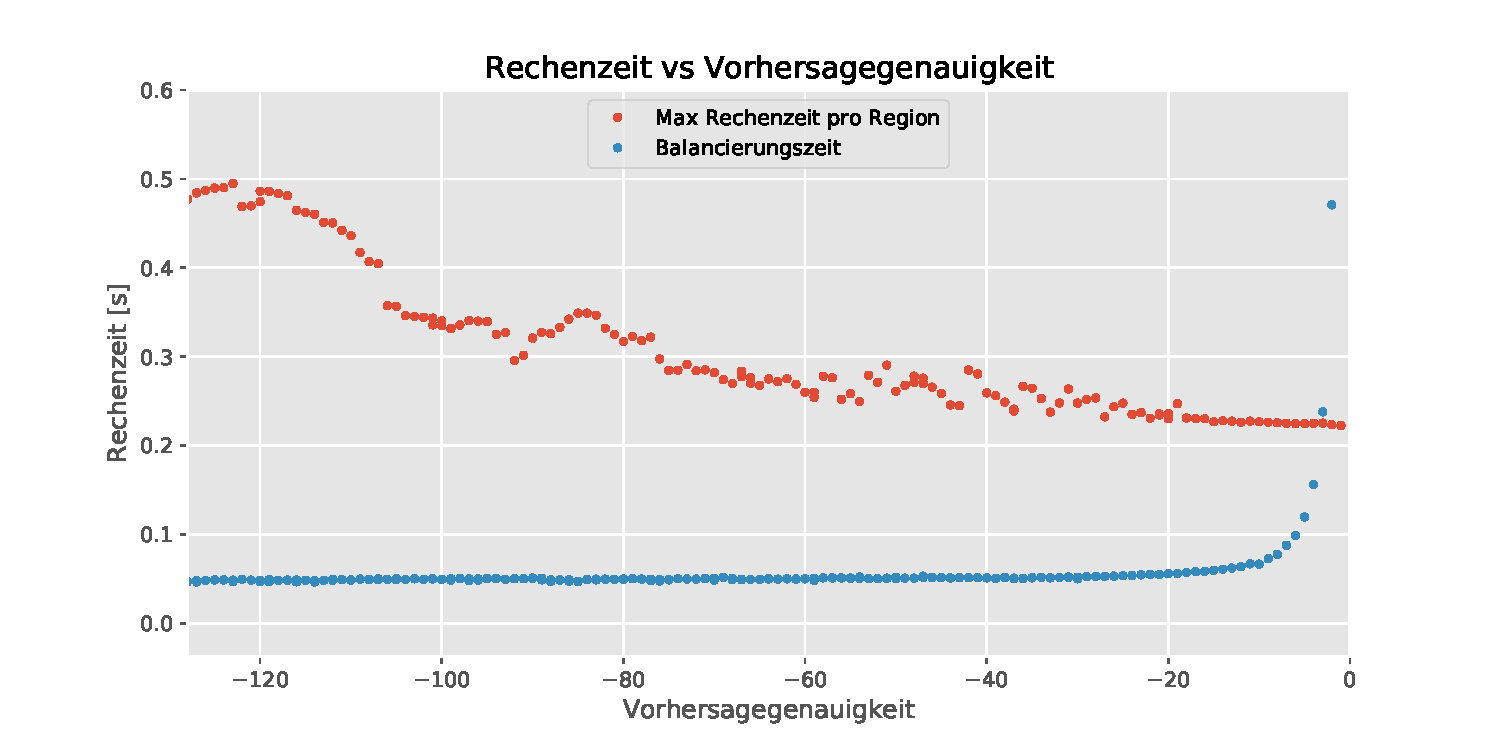
\includegraphics[width=0.9\linewidth]{img/Evaluation/prediction_accuracy_tile2_cropped.pdf}
	\caption{Maximale Rechenzeit pro Region im Vergleich zur benötigte Zeit für die Vorhersage für verschiedene Vorhersagegenauigkeiten bei minimaler Teilbarkeit von 2.
		Eine Vorhersagegenauigkeit von $1$ bzw. $-1$ ist genau eine Vorhersage pro 2x2-Kachel. Eine negative Zahl bedeutet eine Vorhersage für mehrere Kacheln. Eine positive Zahl bedeutet mehrere Vorhersagen für eine Kachel.}
	\label{fig:balancers_prediction_accuracy}
\end{figure}

In \autoref{fig:balancers_prediction_accuracy} sieht man, dass die maximale Rechenzeit bereits ab einer Genauigkeit von
einer Stichprobe pro 400 2x2-Kacheln (d.h. Genauigkeit -20), also 1600 Pixeln nicht mehr signifikant fällt.
Die für die Lastbalancierung benötigte Zeit steigt exponentiell an, da jede Erhöhung der Genauigkeit um 1 eine Verdopplung der zu berechnenden Pixel bedeutet.
Jedoch erst recht spät, bei einer Genauigkeit von einer Vorhersage pro 1600 Pixeln beginnt dieses Wachstum sichtbar zu werden
und erst bei einer Vorhersage pro 16 Pixeln übersteigt sie die maximale Berechnungsdauer einer Region.

Man sieht auch, dass die maximale Rechendauer manchmal trotz Erhöhung der Genauigkeit ansteigt.
Dies liegt daran, dass für diese Genauigkeiten die Pixel der Vorhersage ungünstig liegen.
Zum Beispiel könnte ein Bereich, der laut Vorhersage außerhalb der Mandelbrotmenge liegt, tatsächlich zum größten Teil in der Menge liegen.
Die Vorhersage ist also nicht repräsentativ für den von ihr abgedeckten Bereich, was zu einer schlechteren Aufteilung führt.

Damit kann beobachtet werden, dass in diesem Fall Lastbalancierung bis zu einem hohen Grad an Genauigkeit nützlich ist
und die Gesamtrechendauer effektiv senken kann.
Dies ist zu erwarten, da für die Berechnung einer geringer aufgelösten Region
der Rechenaufwand im zweidimensionalen quadratisch sinkt.

%% TODO folgenden absatz einbauen --> ist bereits in Implementierung, haben wir ja auch währenddessen festgestellt
% Probleme bei der Verwendung des Rekursiven Lastbalanierers:
% Da es stets im Diskreten eine Minimalgröße für die aufgeteilten Regionen gibt,
% kann es sein, dass eine Region für die eine hohe Last vorhergesagt wird viele Worker reserviert -
% diese jedoch nicht vollständig ausreizen kann, da die Maximalaufteilung schon erreicht wurde.
% Durch die dadurch entstehenden Leerregionen von nicht verwendbaren Workern
% kann eine suboptimale Aufteilung enstehen, schlechter noch als die des naiven rekursiven Balancierers.
%
% Dies kann abgeschwächt werden, indem eine Region stets nur soviel Workerressourcen erhält,
% wie sie maximal auslasten könnte (Fläche/Fläche minimaler Aufteilung)
